\newcommand{\jp}{j^\prime}
\newcommand{\jpp}{j^{\prime\prime}}
\newcommand{\lp}{l^\prime}
\newcommand{\lpp}{l^{\prime\prime}}
\newcommand{\fc}{\bm{\Phi}\genfrac{(}{)}{0pt}{}{j \jp}{l \lp}}
\newcommand{\fczero}{\bm{\Phi}\genfrac{(}{)}{0pt}{}{j \jp}{0 \lp}}
\newcommand{\fcb}{\bm{\Theta}\genfrac{(}{)}{0pt}{}{j \jp}{l \lp}}
\newcommand{\fcbpp}{\bm{\Theta}\genfrac{(}{)}{0pt}{}{j \jpp}{l \lpp}}
\newcommand{\fcbf}{-\bm{\Theta}\genfrac{(}{)}{0pt}{}{j \jp}{l \lp} + \delta_{j,\jp} \delta_{l,\lp} \sum_{\jpp, \lpp}  \bm{\Theta}\genfrac{(}{)}{0pt}{}{j \jpp}{l \lpp} }
\newcommand{\rla}[1]{\langle #1 \rangle}
\newcommand*\tageq{\refstepcounter{equation}\tag{\theequation}}

\chapter{Methods}\label{ch:method}

\section{Neutron Scattering}\label{sec:neutron}
In this section, we give some of the key equations and concepts related to neutron scattering. Basic concepts will not be dealt with in detail, since excellent literature already exists and does a much better job than I would be capable of. See e.g. \cite{Lovesey1984, Squires2012, Schober2014} for general theory and \cite{Shirane2002} for triple-axis spectroscopy. Rather, I will attempt to take a more practical approach with three primary goals:

\begin{enumerate}
	\item Understand what types of problems can be solved with neutron scattering.
	\item Understand the concept of correlation functions and why they are essential to neutron scattering.
	\item Outline the equations \emph{actually} used when performing experiments and comparing with theory.
\end{enumerate}

\subsection{General Theory}
In neutron scattering, the idea is to illuminate a sample with a beam of neutrons and then record the scattered neutrons. In order to have enough neutrons for our experiments, they are usually produced through nuclear fission in a reactor or by bombarding a target with high energy protons in a so-called spallation source.

\begin{table}
	\caption[Neutron Temperatures]{Approximate values of of energies, temperatures and wavelength for the three classifications of reactor sources. From \cite{Squires2012}.}
	\label{fig:neutron_temperatures}
	\centering
	\begin{tabular}{@{}llll@{}}
		\toprule
		Source  & Energy [meV] & Temperature [K] & Wavelength [\AA]  \\ \midrule
		cold    & 0.1-10       & 1-120           & 30-3               \\
		thermal & 5-100        & 60-1000         & 4-1                \\
		hot     & 100-500      & 1000-6000       & 1-0.4              \\ \bottomrule
		\end{tabular}
\end{table}

The neutron is a neutral, spin-$\frac{1}{2}$ particle with a mass $m_\text{n} = \SI{1.675e-27}{\kilo\gram}$ and a magnetic moment $\mu_\text{n} = -1.913 \, \mu_\text{B}$. Just like any quantum object, the neutron exhibits particle-wave duality and as it propagates through a medium we can conveniently characterize it by a wavevector $\bm{k}$ that has a magnitude $k = \frac{2\pi}{\lambda}$, where $\lambda$ is the wavelength, and points in the direction of propagation. Given the wavevector $\bm{k}$, along with the fact that typical neutrons for experiments can be treated as non-relativistic particle, we can compute the neutron energy $E = \frac{\hbar^2 k^2}{2m_\text{n}}$ and its equivalent temperature through $E = k_\text{B}T$. In neutron scattering we often categorize experimental methods based on the temperature of the incident neutrons, as summarized in table \ref{fig:neutron_temperatures}. 

In general, scattering experiments have optimal conditions when the wavelength of the probe is similar to the studied length scale. Similarly, when studying excitations, it is preferable that the energy of the probe is similar to that of the excitations. This is exactly why neutron scattering is so useful for condensed matter since typical wavelengths matches interatomic distances ($\approx \SI{e-10}{\meter}$) and typical energies matches elemental excitations of matter ($\approx \SI{10}{\milli\eV}$). In addition, since the neutron has a magnetic moment it can be used to study magnetic structure and excitations.

In order to describe the scattering experiment, we first need to understand how the neutron interacts with the atomic species in our sample. The process is a neutron-nucleus scattering process, where the potential of the nucleus is approximated by the Fermi pseudopotential
%
\begin{equation}\label{eq:fermi_pseudopotential}
V(\bm{r}) = \frac{2\pi \hbar}{m_\text{n}} b \delta (\bm{r}) \, ,
\end{equation}
%
where $b$ is called the \emph{nuclear scattering length} and depends on the specific nuclear species involved in the scattering process. The $\delta$-function in the pseudopotential is an expression of the fact that we are using the \emph{Born approximation}, which is essentially a statement that the nucleus can be thought of as a point-scatterer compared to the neutron. Since the wavelength of a typical thermal neutrons ($\approx \SI{e-10}{\meter}$) is orders of magnitude larger than the range of nuclear forces ($\approx \SI{e-15}{\meter}$), this is a reasonable assumption. For a single, free nuclei, the scattering will be isotropic and the total scattering is $\sigma_\text{tot} = 4\pi b^2$.

The general geometry of a scattering experiment is outlined in figure \ref{fig:dsdo_geometry}. An incident beam with wave vector $k_\text{i}$ is scattered from the origin to a final wave vector $k_\text{f}$ at an azimuthal angle $\Theta$ and a polar angle $\Phi$ into a solid angle $\Omega$ distance $r$ away from the origin. From this geometry we define the differential scattering cross-section as
%
\[ \frac{\mathrm{d} \sigma}{\mathrm{d}\Omega} = \frac{\text{flux of neutrons into } \mathrm{d}\Omega}{\text{incident flux of neutrons}} \]
%
Since we can only measure the neutron flux, $\mathrm{d}\sigma / \mathrm{d}\Omega$ is our experimental observable, given that we have neutron detectors before and after the sample. Since the neutron flux tells us nothing about the wave vectors or energy, additional constraints are necessary to get information about the scattering process from the experiment. In \emph{elastic scattering}, we assume that no energy is exchanged in the scattering process so that $|\bm{k}_\text{f}| = |\bm{k}_\text{i}|$. By fixing one of them (typically $\bm{k}_\text{i}$), the other is completely described by the geometry of figure \ref{fig:dsdo_geometry} and we can measure $\mathrm{d}\sigma / \mathrm{d}\Omega$ as a function of $\bm{k}_\text{f}$ since the location of our detector, and thus $\Phi$ and $\Theta$ is known. In \emph{inelastic scattering}, we need to fix the lengths, and thus the energy, of both $\bm{k}_\text{i}$ and $\bm{k}_\text{f}$. This defines the \emph{partial differential cross-section}:
%
\[ \frac{\mathrm{d}^2 \sigma}{\mathrm{d}\Omega \mathrm{d}E_\text{f}} = \frac{\text{flux of neutrons into } \mathrm{d}\Omega \text{ with energy between } E_\text{f} \text{ and } E_\text{f} + \mathrm{d}E_\text{f}}{\text{incident neutron flux with energy } E_\text{i}} \, , \]
%
where $E_\text{i}$ is the energy of the incident neutron and $E_\text{f}$ is the energy of the final neutron. How to technically achieve neutron beams with fixed wave vectors will be described later on in the relevant experimental sections, but for now we just make the assumption that it is possible. With the observables now defined, we can start to discuss how to actually extract useful information about the atomic/microscopic details of a sample from a neutron scattering experiment. Knowing $\bm{k}_\text{i}$ and $\bm{k}_\text{f}$, the coordinate system can be redefined with respect to our sample through the scattering vector $\bm{Q} = \bm{k}_\text{i} - \bm{k}_\text{f}$. In addition, we define the \emph{energy transfer} as the amount of energy gained (or lost, for negative values) by the neutron in the scattering process $\hbar \omega = E_\text{f} - E_\text{i}$.

\begin{figure}
	\centering
	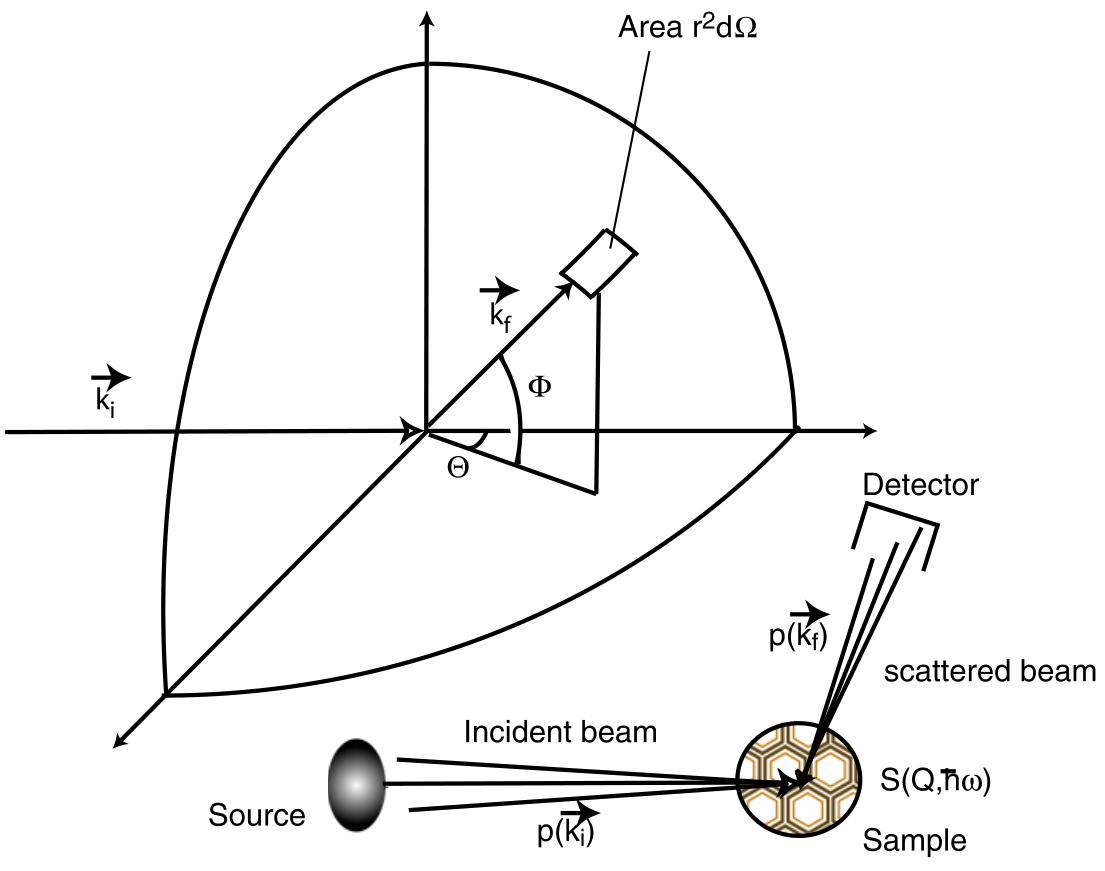
\includegraphics[width=0.6\textwidth]{fig/method/ns/dsdo_schober.png}
	\caption[scattering cross-section geometry]{Geometry of a scattering experiment. An incident beam of neutrons characterized by the wave vector $\bm{k}_\text{i}$ impinges on a sample at the origin. The neutron beam is scattered in the direction of $\bm{k}_\text{f}$, defined by the two angles $\Phi$ and $\Theta$. The neutrons are detected at a solid angle $\mathrm{d}\Omega$ at a distance $r$. From \cite{Schober2014}}
	\label{fig:dsdo_geometry}
\end{figure}

The objective of neutron scattering theory (or really, any scattering theory), is then to find a sample-dependent function $S(\bm{Q}, \omega)$ that can be related to the observable (partial) scattering cross-section. In fact, as we shall see in the next section, it turns out that this \emph{scattering function} $S(\bm{Q}, \omega)$ not only exists, but have an intimate relationship with microscopic correlation functions which can be derived from first principles. 

This, somewhat abstract, introduction essentially covers most of what we need to know with regards to the neutron scattering process and coordinate systems. The rest of this section is then dedicated to 1) understanding what the scattering function $S(\bm{Q}, \omega)$ actually represents and 2) outline some of practicalities involved in the neutron scattered methods used in this thesis. 

\subsection{Correlation Functions}
After setting up the coordinate system, we are now left with the much more complicated task of constructing models that can help is interpret the partial differential cross-section. As I previously suggested, information about our samples comes from the pattern of $\mathrm{d}^2 \sigma / \mathrm{d}\Omega \mathrm{d}E_\text{f}$ as a function of $\bm{Q}$ and $\omega$, or equivalently: The angles $\Phi$, $\Theta$ and neutron energies $E_\text{i}$, $E_\text{f}$. Intuitively, the reason we have any pattern  at all is due to interference of the scattered waves. Since the scattering from a single nucleus is isotropic, any pattern in $S(\bm{Q}, \omega)$ comes from the specific composition of, or correlations between, atomic species in our sample. 

It turns out that this can be conveniently described through the mathematics of correlation functions, introduced by \citeauthor{VanHove1954} in 1954 \cite{VanHove1954}. We start with the \emph{time-dependent pair-correlation function} for a system of identical particles $G(\bm{r}, t)$, which describes the probability of finding a pair of particles separated by the spatial vector $\bm{r}$ at time $t$. Similarly, the \emph{self time-dependent pair-correlation function} $G_\text{s}(\bm{r}, t)$ describes the probability of finding the same particle at a distance $\bm{r}$ at a time $t$. These concepts are illustrated in figure \ref{fig:correlation_functions}\todo{probably remove this if no time} and can be defined mathematically defined through position operators:

\begin{figure}
	\centering
	\missingfigure{correlation functions illustration}
	\caption[pair correlation functions]{pair correlation functions}
	\label{fig:correlation_functions}
\end{figure}

\begin{align*}
	G(\bm{r}, t) &= \frac{1}{N} \sum_{i \neq j} \int \left\langle  \delta (\bm{r}^\prime - \bm{R}_j(0) ) \delta (\bm{r}^\prime + \bm{r} - \bm{R}_i(t)) \right\rangle \mathrm{d}\bm{r}^\prime \\
	G_\text{s}(\bm{r}, t) &= \frac{1}{N} \sum_{i} \int \left\langle  \delta (\bm{r}^\prime - \bm{R}_i(0) ) \delta (\bm{r}^\prime + \bm{r} - \bm{R}_i(t)) \right\rangle \mathrm{d}\bm{r}^\prime \, ,
\end{align*}

\noindent where $i$, $j$ are particle indices and $\bm{R}_i(t)$ is the position operator for particle $i$ at time $t$. Finally the following functions can be obtained through Fourier transforms in time and space:

\begin{align*}
	I(\bm{Q}, t) &= \int G(\bm{r},t) \exp (i \bm{Q} \cdot \bm{r} ) \mathrm{d}\bm{r} \\
	I_\text{s}(\bm{Q}, t) &= \int G_\text{s}(\bm{r},t) \exp (i \bm{Q} \cdot \bm{r} ) \mathrm{d}\bm{r} \\
	S(\bm{Q}, \omega) &= \frac{1}{2 \pi \hbar} \int I(\bm{Q}, t) \exp (-i \omega t) \mathrm{d}t \, \\
	S_\text{i}(\bm{Q}, t) &= \frac{1}{2 \pi \hbar} \int I_\text{s}(\bm{Q}, t) \exp (-i \omega t) \mathrm{d}t \, ,
\end{align*}

\noindent where $I(\bm{Q}, t)$ is known as the \emph{intermediate function}, $I_\text{s}(\bm{Q}, t)$ the \emph{self intermediate function}, $S(\bm{Q}, \omega)$ the \emph{scattering function} and $S_\text{i}(\bm{Q}, t)$ the \emph{incoherent scattering function}. The connection to the partial differential cross-section can now be stated succinctly as

\begin{equation}
	\frac{\mathrm{d}^2\sigma}{\mathrm{d}\Omega\mathrm{d}E_\text{f}} = \left( \frac{\mathrm{d}^2\sigma}{\mathrm{d}\Omega\mathrm{d}E_\text{f}} \right)_\text{coh} + \left( \frac{\mathrm{d}^2\sigma}{\mathrm{d}\Omega\mathrm{d}E_\text{f}} \right)_\text{inc} \\
\end{equation}

\noindent with

\begin{align*}
	\left( \frac{\mathrm{d}^2\sigma}{\mathrm{d}\Omega\mathrm{d}E_\text{f}} \right)_\text{coh} &= \frac{\sigma_\text{coh}}{4\pi}\frac{k_\text{f}}{k_\text{i}}N S(\bm{Q}, \omega) \\ 
	\left( \frac{\mathrm{d}^2\sigma}{\mathrm{d}\Omega\mathrm{d}E_\text{f}} \right)_\text{inc} &= \frac{\sigma_\text{inc}}{4\pi}\frac{k_\text{f}}{k_\text{i}}N S_\text{i}(\bm{Q}, \omega)
\end{align*}

\noindent where

\begin{align*}
	\sigma_\text{coh} &= 4 \pi \overline{b}^2 \\
	\sigma_\text{inc} &= 4 \pi \left( \overline{b^2} - \overline{b}^2 \right)
\end{align*}

\noindent In the above equations, $N$ is the number of particles in the scattering system, $b$ is the nuclear scattering length as defined in equation \eqref{eq:fermi_pseudopotential} and the bars denote ensemble averages. The \emph{coherent cross-section} $\sigma_\text{coh}$ is thus related to the average scattering length, while the \emph{incoherent cross-section} $\sigma_\text{inc}$ is related to the distribution of scattering lengths. These cross-sections are determined experimentally and are tabulated for most elements \cite{nist}.

In a neutron scattering experiment we thus see a superposition pair-correlations through coherent scattering and self-correlations through incoherent scattering. As an example involving dynamics, phonons (correlated motion) are generally seen as coherent scattering while Brownian motion (random motion) would show up as incoherent scattering.

It thus turns out that there is a direct relationship between the measured partial differential cross-section in neutron scattering and microscopic correlation functions. In fact, many microscopic theories can be translated directly into a theoretical $S(\bm{Q}, \omega)$ and compared 1-to-1 with experiment. One illustrative example, used in this thesis, is that of a molecular dynamics simulation where we record the atomic positions as a function of time. From this trajectory it is trivial to compute a classical version of $G(\bm{r},t)$ and thus obtain predictions for neutron scattering experiments.

Even more generally, given a Hamiltonian (quantum or classical) and assuming a weak (linear) perturbation, it is possible to invoke linear response theory (see e.g. \cite[chapter 3]{Jensen1991}). Importantly, linear response theory provides a link between the spontaneous fluctuations of a system and the response to an external perturbation. The object of interest in this context becomes the dynamic susceptibility $\chi(\bm{Q}, \omega)$, which can be thought of as
%
\[ \chi(\bm{Q}, \omega) = \chi^{\prime}(\bm{Q}, \omega) + \chi^{\prime\prime}(\bm{Q}, \omega) = \frac{\text{`response'}}{\text{`force'}} \, , \]
%
where the real part $\chi^{\prime}(\bm{Q}, \omega)$ describes a response in phase with the perturbation (reactive),
while the imaginary part $\chi^{\prime\prime}(\bm{Q}, \omega)$ describes an anti-phase response (dissipative). The real and imaginary parts are linked through the Kramers-Kronig relation
%
\[ \chi^{\prime\prime}(\bm{Q}, \omega) = - \frac{1}{\pi} \mathcal{P} \int_{-\infty}^{\infty} \frac{\chi^{\prime}(\bm{Q},\omega^\prime)}{\omega^\prime - \omega} \mathrm{d}\omega^\prime \, , \]
%
where $\mathcal{P}$ is the Cauchy principal value. Finally, the scattering function is related to the imaginary part of dynamic susceptibility through the fluctuation-dissipation theorem:
%
\[ S(\bm{Q},\omega) = \frac{1}{1-e^{\frac{\hbar\omega}{k_\text{B}T}}} \chi^{\prime\prime}(\bm{Q}, \omega) \, . \]
%
Since the real and imaginary parts of the susceptibility are uniquely connected through the Kramers-Kronig relation, neutron scattering experiments can directly probe predictions of linear response theory. A particularly illustrative example\todo{maybe remove this or put in appendix} in the context of this thesis is that of a damped harmonic oscillator (DHO). Consider the classical system shown in figure \ref{fig:dho_chi}, with the equations of motion:

\begin{figure}[]
	\centering
	\inputTikZ{0.8}{fig/method/ns/dho.tex}\hspace{4mm}
	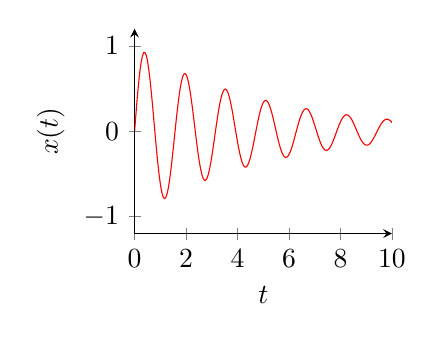
\begin{tikzpicture}
		\pgfplotsset{width=0.4\textwidth}
		\begin{axis}[xlabel=$t$, ylabel=$x(t)$, axis lines = left, ymin=-1.2, ymax=1.2]
			\addplot[color=red, domain=0:10, range=-1:1, samples=200]{exp(-0.2*x)*sin(deg(4*x))};
		\end{axis}
	\end{tikzpicture}
	\caption[DHO schematic]{Mechanical version of the damped harmonic oscillator. \textbf{Left:} A mass on a spring moving with velocity $\bm{v}$ under the influence of a restoring spring force (blue arrow) with force constant $\omega_0^2$ and a frictional force $\gamma$ which is linear in velocity. \textbf{Right:} Position of the spring as a function of time after applying a an impulsive perturbation, analogous to quickly pulling the mass and letting go.}
	\label{fig:dho_chi}
\end{figure}

\[ m \rla{\ddot{x}(t)} + m w_0^2 \rla{x(t)} = - m\gamma\rla{\dot{x}(t)} \, . \]

\noindent Assuming an impulsive perturbation and going through the mathematics of linear response theory (see \cite{Lovesey1984} for details), we arrive at the dynamic susceptibility
%
\[ \chi[\omega] = \frac{1}{m}\frac{1}{\omega_0^2 - \omega^2 + i\gamma\omega} = \frac{1}{m} \frac{\omega_0^2 - \omega^2}{(\omega_0^2-\omega^2)^2 + \gamma^2\omega^2} - \frac{i}{m}\frac{\gamma\omega}{(\omega_0^2-\omega^2)^2 + \gamma^2\omega^2} \, . \]
%
From the last term we thus see that damped harmonic motion can be observed as a Lorentzian as a function of energy in a neutron scattering experiment, where the position $\omega_0$ denotes the fundamental frequency and the width $\gamma$ is the damping constant. In fact, this expression is typically used as a fitting function when measuring phonons \cite{Fak1997}. While rudimentary, the purpose of this example is to emphasize the intimate relationship between observables in neutron scattering and microscopic theories.

\subsection{Resolution}
Maybe a short section about resolution? Just basic concepts starting from distributions of neutron beams.

\section{Specific Scattering Methods}\label{sec:specific_neutron}
Departing from the abstract concepts of the preceding section, I will now outline specific neutron scattering techniques used in the experimental part of this thesis. Despite the significant power generated in a neutron reactor, the number of neutrons expelled from the source is typically small with respect to neutron experiments, especially when compared to X-ray synchrotron radiation\todo{some numbers}. In addition, the neutrons have a wide distribution of wavelengths and propagate in all directions. Neutron facilities and instruments thus take advantage of various optical elements in order to define the neutron beam.

Transporting the neutrons to the instruments is done with neutron guides, which are rectangular tubes where the insides are coated with mirrors that can cause total reflection of neutrons at sufficiently small angles. When the neutrons reach the instrument, we have so-called \emph{white beam} with a wide distribution of wavelengths, but most experiments needs a well-defined $\bm{k}_\text{i}$. For this we use a \emph{monochromator}, which is a crystalline material that takes advantage of Bragg scattering. Similarly, if we want a well-defined final neutron energy, we can place an identical element (an \emph{analyser}) before our detector.

Neutron instruments are complicated and discussing them in detail would divert from the main purpose of understanding how to use them. For now, it will suffice to know that we have found a way to build neutron scattering instruments such that the geometry in figure \ref{fig:dsdo_geometry} is valid. Other details will be discussed where appropriate.

\subsection{Triple-Axis Spectroscopy}

\begin{figure}
	\centering
	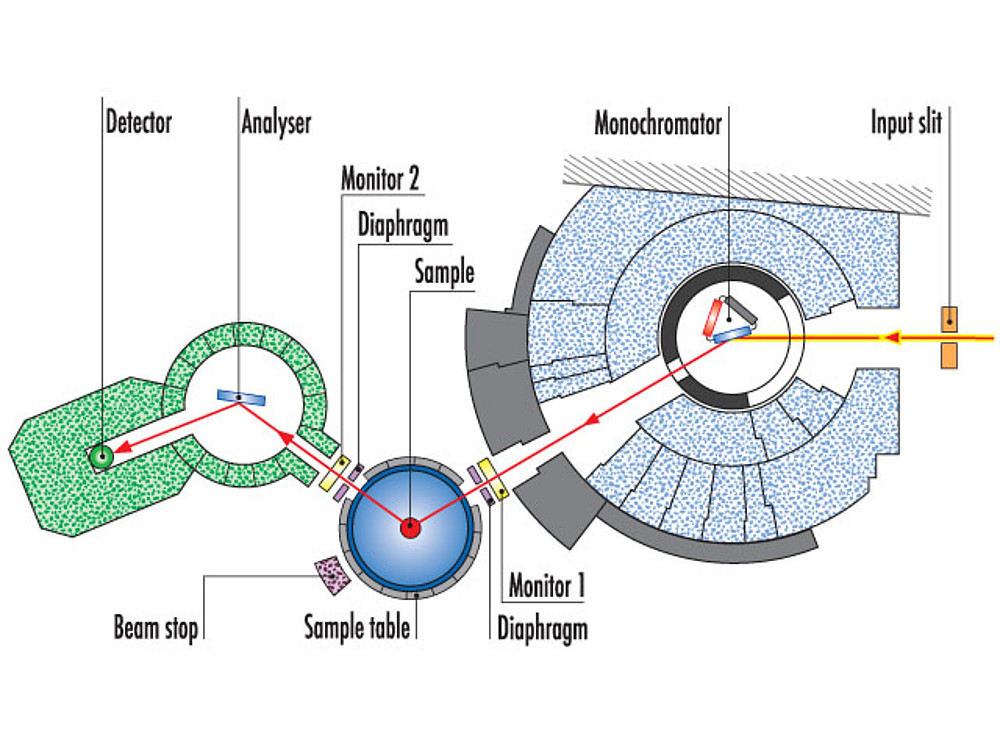
\includegraphics[width=0.6\textwidth]{fig/method/ns/in8.jpg}
	\caption[in8 layout]{Layout of the IN8 instrument at ILL \cite{in8}. Neutrons from the thermal source hits one of the 3 optional monochromators (PG002, Cu200, Si111) and continues towards the sample where it is scattered towards the analyser that selects the final energy.}
	\label{fig:in8}
\end{figure}

In some way, the triple-axis spectrometer (TAS) is the easiest neutron scattering instrument to understand because it has a one-to-one correspondence with the geometry from figure \ref{fig:dsdo_geometry}. Figure \ref{fig:in8} shows the view from above of the TAS instrument IN8 at ILL. The triple-axis (or triple-angle) name comes from the fact that all the angles defined by the beam path can be adjusted by moving the motors of the instrument. These angles then completely define $\bm{k}_\text{i}$, $\bm{k}_\text{f}$ and we essentially have a two dimensional version of figure \ref{fig:dsdo_geometry}, known as the \emph{scattering plane}.

Because the instrument is essentially two-dimensional, single crystal samples must be aligned with a desired crystal plane in the scattering plane. For the cuprates, we typically have tetragonal (or almost-tetragonal) crystal structures so we typically align in the $a$-$b$ or $a$-$c$ plane. With the sample in place, we can now completely explore $S(\bm{Q},\omega)$ with the restriction that $\bm{Q}$ is restricted to the scattering plane. The sample is placed on a rotating sample stick that, together with the scattering angle, allows us to access the two dimensions of $\bm{Q}$. The energy transfer $\hbar\omega$ is controlled by monochromator and analyser.

As one might have noticed, figure \ref{fig:in8} features just a single detector. While other options exists (see chapter \ref{ch:lowen}), this is typical for TAS instruments. As a consequence, measurements are performed along pre-defined paths in $(\bm{Q}, \omega)$ space step-by-step. The main purpose of TAS instruments is then generally to look at specific features in $S(\bm{Q},\omega)$ with high counting statistics and tight resolution. Since inelastic scattering is orders of magnitude weaker than elastic scattering, spectroscopic measurements are usually the primary focus for TAS instruments.

In this thesis, most TAS measurements are of specific phonon branches. The 1-phonon cross-section gives an expression for the differential cross section of phonons, indexed by phonon band.

\begin{equation}
	S(\bm{Q},\nu,\omega) = \frac{k_\text{f}}{k_\text{i}} \frac{N}{\hbar} \sum_{\bm{q}} | F(\bm{Q},\bm{q},\nu) |^2 ( n_{\bm{q}\nu} + 1) \delta (\omega - \omega_{\bm{q}\nu}) \delta(\bm{Q} - \bm{q} - \bm{G})
	\label{eq:one_phonon_sqw}
\end{equation}
%
with
%
\[
	F(\bm{Q}, \bm{q}, \nu) = \sum_j \sqrt{\frac{\hbar}{2 m_j \omega_{\bm{q}\nu}}} \bar{b}_j \exp \left( -\frac{1}{2} \langle | \bm{Q} \cdot \bm{u}(j0) |^2 \rangle \right) \exp [ -i(\bm{Q} - \bm{q}) \cdot \bm{r}(j0) ] \bm{Q} \cdot \bm{e}_j(\bm{q},\nu)
\]
%
where $\bm{Q}$ and $\omega$ are the wave vector and energy of our measurement. $\nu$ is a phonon band and $\bm{q}$ is a wave vector. $\omega_{\bm{q}\nu}$ is the energy of phonon band $\nu$ at wave vector $\bm{q}$ and $n_{\bm{q}\nu}$ is the Bose factor at this energy. Atomic species are designated with index $j$, their mass is $m_j$ and their coherent neutron cross-section is $\bar{b}_j$. $\bm{u}(j0)$ and $\bm{r}(j0)$ is the displacement and position of atom $j$ in unit cell 0, respectively. Finally, $G$ is any reciprocal lattice vector and $\bm{e}_j(\bm{q},\nu)$ is the phonon eigenvector of atom $j$, band $\nu$ and wave vector $\bm{q}$.

While this expression rests on some microscopic details that we might not have knowledge of, close inspection of equation \eqref{eq:one_phonon_sqw} allows us to extract information from an experiment without any prior knowledge of the system. The $\delta$-functions makes sure that we only see scattering at the phonon dispersion. In addition, the $\bm{Q}\cdot \bm{e}_j(\bm{q},\nu)$ term tells us that scattering is strongest when the eigenvector of the phonon mode is parallel to $\bm{Q}$ (and vanishes when perpendicular). This allows us to distinguish longitudinal and transverse phonons.

As it turns out, it \emph{is} possible to obtain prior knowledge about the phonon spectrum through microscopic simulations. These simulations give us direct access to eigenvectors and we can make a detailed analysis of equation \eqref{eq:one_phonon_sqw}. More information about this type of calculation is given in section \ref{sec:phonon_calc}.

\subsection{Time-of-Flight Spectroscopy}

\begin{figure}
	\centering
	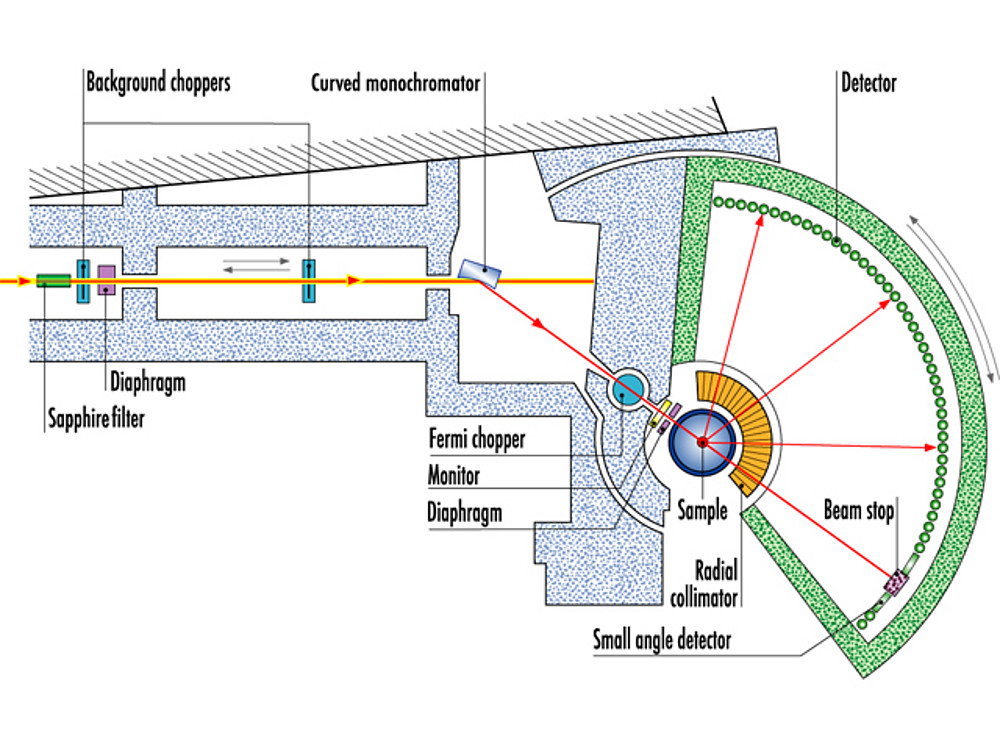
\includegraphics[width=0.6\textwidth]{fig/method/ns/in4.jpg}
	\caption[in4 layout]{Layout of the IN4 instrument at ILL \cite{in4}. Neutrons are chopped into discrete packets before hitting the monochomator and continuing towards the sample position. A Fermi chopper is used to make very short neutron pulses, such that their $(Q,\omega)$ can be determined from the time-of-flight from the Fermi chopper to the detector,}
	\label{fig:in4}
\end{figure}

In Time-of-Flight (ToF) spectroscopy, we take advantage of the fact that thermal neutrons move at speeds that we can accurately determine experimentally (\SI{10}{\milli\eV} neutrons has a speed of roughly \SI{1400}{\meter\per\second}). Figure \ref{fig:in4} shows a schematic of the IN4c spectrometer at ILL. Neutrons from the reactor are chopped up into discrete packets using two rotating discs (background choppers) and then monochromatized using a crystal monochromator. Before impinging on the sample, the neutrons pass through a `Fermi chopper' which produces very short neutron pulses (\SIrange{10}{50}{\micro\second}). Neutrons are then detected radially in one of the many detectors. By recording the time-of-flight from the Fermi chopper to a specific detector, we can determine the energy transfer through the velocity as determined from the flight time and $\bm{Q}$ from the angle to the detector where the neutron was measured.

Time-of-Flight spectrometers thus perform many simultaneous measurements, but can in some sense be used to probe many of the same things as TAS instruments. The better choice depends, of course, on the sample and phenomena that you are using it to probe. In the case of this thesis, we used the IN4 spectrometer to measure the phonon density-of-states of powdered samples. Since the powder is rotationally averaged, the result of a measurement is a $(Q,\hbar\omega)$ map where $Q$ is defined as the length of $\bm{Q}$. An example of such a dataset is shown in figure \ref{fig:sample_sqw} in chapter \ref{ch:in4}. By integrating the full map onto the energy axis we obtain the experimental phonon density-of-states.

While equation \ref{eq:one_phonon_sqw} is still valid since most of our scattering is 1-phonon processes at low temperature, we use the confusingly named \emph{incoherent approximation}. The physical reasoning is that the rotational averaging due to the powder cancels out correlations between distinct atoms. Mathematically, it is due to factor 
%
\[ \left( \sum_j \bm{Q} \cdot \bm{e}_j (\bm{q}, \nu) \right)^2 \, \]
%
which in the incoherent approximation is replaced by \cite{Carpenter1985}\todo{I think this is correct, not 100\% sure}
%
\[ \sum_j  Q^2 \left( \bm{e}_j (\bm{q}, \nu) \right)^2 \]
%
essentially eliminating the cross terms. With this approximation, the 1-phonon incoherent cross-section becomes\todo{check these equations and make consistent with notation}:
%
\[ S^{(1)}_{\mathrm{inc}}(Q,E) = \exp\left(-2\bar{W}(Q)\right) \frac{Q^2}{E} \langle n+\frac{1}{2}\pm\frac{1}{2} \rangle \left[ \sum_k \frac{\sigma_k^{\mathrm{scatt}}}{2m_k} g_k(E) \right]\, \]
%
where $g_k(E)$ represents the phonon density of states. With this, much simpler, expression we can transform our $(Q,E)$ dataset into the phonon density of states, only supplying the mean-squared displacement and atomic composition. Similar to the phonon bands, the phonon density of states can also be directly obtained from simulations methods. ToF spectroscopy on powders thus allows us to investigate properties of the overall phonon spectra, in contrast to the distinct phonon bands as measured by TAS spectroscopy.

\subsection{Real-space diffraction}

\begin{figure}
	\centering
	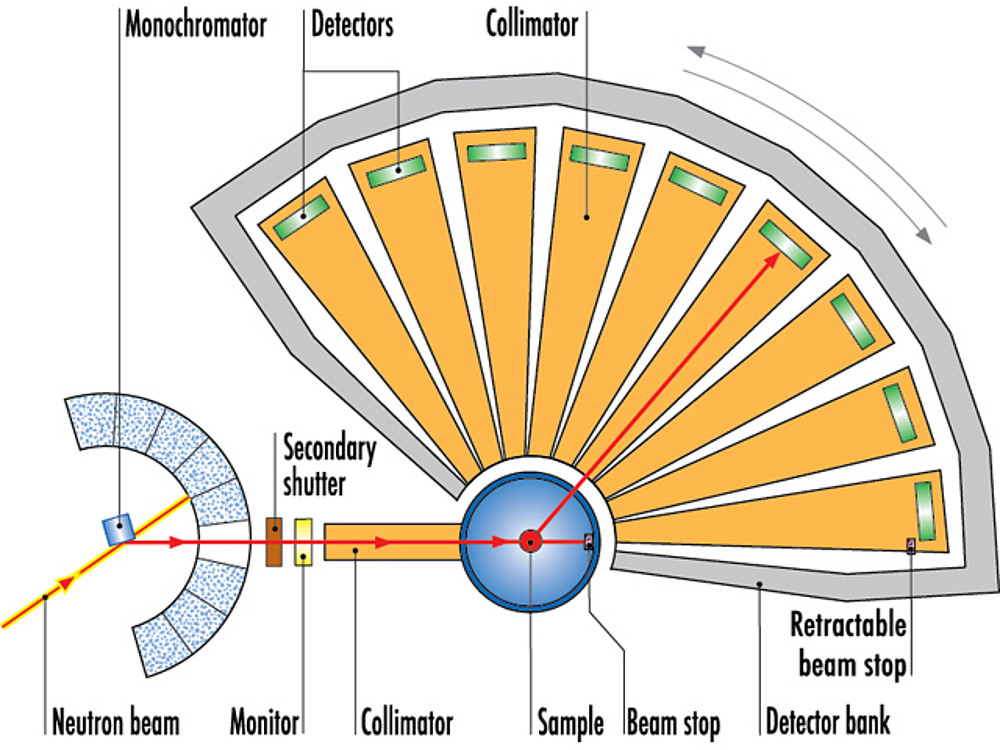
\includegraphics[width=0.6\textwidth]{fig/method/ns/d4.jpg}
	\caption[D4 layout]{Shcematic layout of the D4 instrument at ILL \cite{d4}. The neutron beam from the hot source hits the monochromator and directed towards the sample position. The scattered neutrons are collected at the nine detectors each containing 64 cells. The detector bank can be moved during the experiment in order to cover the full $Q$-range.}
	\label{fig:d4}
\end{figure}

The last method I will cover here is a diffraction instrument focussed on obtaining real space structures. In terms of the correlation functions defined in section \ref{sec:neutron}, we are interested in the time-averaged value of $G(\bm{r}, t)$ which can be found as the Fourier transform of $S(\bm{Q},\omega=0)$. In order to perform this Fourier transform, it is desired to measure at a wide range of $\bm{Q}$ in order to avoid artefacts related to the Fourier transformation pocedure itself.

Figure \ref{fig:d4} shows the D4 diffractometer at ILL. Since diffraction assumes elastic scattering, the instrument is equipped with a monochromator before the sample, but no energy analysis of the scattered neutrons is performed. Rather, the neutrons are directly measured at the radial detectors. In order to optimize the $\bm{Q}$-range of the instrument, we want to minimize the wavelength (Bragg's law), so D4 is placed at a hot source so that we can get a large number of high-energy neutrons. For our particular experiment the monochromator selected neutrons with a wavelength $\lambda = \SI{0.35}{\angstrom}$, corresponding to an energy of $E = \SI{668}{\milli\eV}$.

The object of interest in this case is the total pair distribution function $G(r)$, which tells you the probability of finding two atoms separated by a distance $r$, weighted by the product of their coherent neutron scattering lengths $\overline{b}$. As we shall see in section \ref{sec:sim_experiment_compare}, these distributions can be found from a molecular dynamics simulation. In order to compare with experiment  we then consider
%
\[ G(r) = \frac{1}{\overline{b}^2} \sum_{\alpha=1,\beta\geq\alpha} c_\alpha c_\beta \overline{b}_\alpha \overline{b}_\beta (g_{\alpha\beta}(r) - 1) \, , \]
%
where $g_{\alpha\beta}(r)$ is the \emph{partial radial distribution function} which describes the probability of finding a particle with label $\beta$ at a distance $r$ away from a particle with label $\alpha$. $c_i = \frac{N_i}{N}$ is the number concentration, $\bar{b_i}$ is the coherent neutron cross section of species $i$,  and 
%
\[ \overline{b}^2 = \left(\sum_\alpha \overline{b}_\alpha c_\alpha \right)^2 \, . \]
%s
In the research community working with pair distribution functions (PDF) there is a large number of conventions regarding how to normalize and represent pair-correlation functions in theory and experiment (see review by \citeauthor{Keen2001} \cite{Keen2001}). The $G(r)$ presented here is typically called the \emph{Total Pair-Distribution Function}, but your mileage may vary. Details about the definitions of $g_{\alpha\beta}(r)$ and $G(r)$ and how to obtain them from molecular dynamics trajectories can be found in section \ref{sec:method_md}

\section{Density Functional Theory}\label{sec:dft}
We now turn to the computational framework used in this thesis, Density Functional Theory (DFT). Similar to the section on neutron scattering, this is a vast subject that is impossible to fully explore on a few pages, but I will once again try to outline the key concepts, advantages and disadvantages. For more comprehensive material, I recommend the books by \citeauthor{Giustino2014} \cite{Giustino2014} (introduction to the subject) and \citeauthor{Martin2004} \cite{Martin2004,Martin2016} (comprehensive reviews). The review paper by \citeauthor{Hoffmann1987} \cite{Hoffmann1987} discusses what kinds of problems DFT can solve and is recommended for anyone curious about DFT.

DFT is a computational method in quantum chemistry, where the objective is to compute the many-body Schr\"odinger equation for molecules and solids:

\begin{equation}\label{eq:mbse}
	\left[ -\sum_i \frac{\nabla_i^2}{2} - \sum_{i} \sum_{I} \frac{Z_I}{|\bm{r}_i - \bm{R}_I|} + \frac{1}{2} \sum_{i \neq j} \frac{1}{|\bm{r}_i - \bm{r}_j|} \right] \Psi = E \Psi \, ,
\end{equation}

\noindent where $\bm{r}_i$ is the position of electron $i$ and $\bm{R}_I$, $Z_I$ is the position, charge of nucleus $I$. As one might have noticed, the kinetic energy of nuclei and nuclei-nuclei interactions have been omitted. This is known as the \emph{clamped nuclei approximation}, which assumes immobile nuclei. This results in a vanishing kinetic energy and a constant coulomb repulsion which can be subtracted from the energy on the right-hand-side of equation \eqref{eq:mbse}:
%
\[ E = E_\text{total} - \frac{1}{2} \sum_{I \neq J} \frac{Z_I Z_J}{|\bm{R}_I - \bm{R}_J|} \]
%
These equations are written in the so-called Hartree units (see \cite[chapter 2.3]{Giustino2014}), such that energies are in units of Hartree energies ($\SI{1}{\hartree} = \SI{27.2114}{\eV}$), distances are in units of the Bohr radius $a_0$ and masses are in units of electron masses $m_e$. Since the nuclear coordinates are considered fixed, the many-body wavefunction $\Psi$ in equation \eqref{eq:mbse} is a function of electron positions
%
\[ \Psi(\bm{r}_1,\bm{r}_2,\dots, \bm{r}_n) \]
%
While this object seems innocent at first glance, the many-body Schr\"odinger equation quickly becomes a completely unmanageable object. Imagine that we want to calculate this object for a small molecule such as Benzene (C$_6$H$_6$) containing 12 nuclei and 42 electrons. This wavefunction exists in $42\cdot3-3 = 123$ dimensional cartesian space! If we want to store this object on a computer with a modest precision of 10 grid points per coordinate, it would require $10^{156}$ complex numbers or $64 \cdot 10^{156}$ bits (assuming single-precision floating points numbers of 32 bits). \citeauthor{Lloyd2002} estimated the total number of bits available for computation in the observable universe to be $10^{90}$ \cite{Lloyd2002}. Even with the entire universe at our disposal this object is completely unmanageable. In order to arrive at a reasonably manageable theory, we assume that electrons are independent such that the many-body wavefunction can be written as a product of single-electron wavefunctions:
%
\begin{equation}\label{eq:independent_electrons}
\Psi(\bm{r}_1,\bm{r}_2,\dots, \bm{r}_n) \longrightarrow \phi_1(\bm{r}_1)\phi_2(\bm{r}_2)\dots\phi_N(\bm{r}_N) \,
\end{equation}
%
Where each of the wavefunctions $\phi_i$ are found as solutions to the single-electron Schr\"odinger equation
%
\[ \left[ - \frac{\nabla^2}{2} - \sum_I \frac{Z_I}{|\bm{r} - \bm{R}_I|} \right] \phi_i = \epsilon_i \phi_i \, . \]
%
Using these definitions, the many-body Schr\"odinger equation becomes
%
\begin{equation}\label{eq:sese}
\sum_i \left[ - \frac{\nabla^2}{2} - \sum_I \frac{Z_I}{|\bm{r}_i - \bm{R}_I|} \right] \Psi = E \Psi \, , 
\end{equation}
%
where $E = \epsilon_1 + \epsilon_2 + \dots \epsilon_N$, with the single-electron energies being ordered from smallest to largest. This corresponds to the situation usually taught in condensed matter physics where the lowest energy configuration is found by filling up electronic orbitals starting from the lowest eigenvalue \cite{Kittel2005}. Inspection of equation \ref{eq:sese} reveals that the independent electron approximation, as the name implies, has completely ignored the Coulomb repulsion between electrons. To rectify this fact, we make a \emph{mean-field approximation}, such that each electrons feels an electrostatic `Hartree potential':
%
\[ \nabla^2 V_H(\bm{r}) = - 4 \pi n(\bm{r}) \, \] 
%
where the electron density is defined as the sum of single-electron densities:

\begin{equation}\label{eq:electron_density}
n(\bm{r}) = \sum_i |\phi_i(\bm{r})|^2 \, .
\end{equation}

\noindent Starting with the many-body Schr\"odinger equation we have thus arrived at an approximate version that can be approached from a computational point of view. However, at this stage we have ignored exchange (equation \eqref{eq:independent_electrons} is not anti-symmetric with regards to a change of variables) and correlation (the mean field approximation used for the Hartree potential). As we shall see, DFT gives us a way to correct for both of these effects in a surprisingly accurate manner.

\subsection{The Kohn-Sham equations}
The main idea behind DFT is expressed through the `Hohenberg−Kohn theorem', which is the simple but powerful statement that the total energy of a many-electron system is a functional of the electron density. In addition, the `Hohenberg–Kohn Variational Principle' tells us that the ground state density is the functional that minimizes the total energy. To quote the original paper \cite{Hohenberg1964}:

\begin{quote}
	This paper deals with the ground state of an interacting electron gas in an external potential $v(\bm{r})$. It is proved that there exists a universal functional of the density, $F[n(\bm{r})]$, independent of $v(\bm{r})$, such that the expression $E= \int v(\bm{r}) n(\bm{r}) \mathrm{d}\bm{r} + F[n(\bm{r})]$ has as its minimum value the correct ground-state energy associated with $v(\bm{r})$.
\end{quote}

\noindent The theorem states the existence of the functional $F[n(\bm{r})]$, but leaves us with no recipe on how to construct this functional. The `game' in DFT thus consists of constructing functionals and test the computational results against experimental observations. Since the universal functional has not been found, hundreds of functionals \cite{Mardirossian2017} have been created with specific purposes in mind. With that being said, very good `universal' functionals exist and most people stick to a small subset of this `functional zoo'. Returning the objective at hand, the idea of \citeauthor{Kohn1965} \cite{Kohn1965} was to split the contributions to the functional $F[n(\bm{r})]$ into terms of kinetic and coulomb energy and an additional term with `everything else':

\begin{align}
	E &= \int V_\text{n}(\bm{r}) n(\bm{r}) \mathrm{d}\bm{r} + F[n(\bm{r})] \label{eq:ks_toten1} \\
	F[n(\bm{r})] &= \sum_i \int \phi_i^*(\bm{r})\frac{\nabla^2}{2}\phi_i(\bm{r}) \mathrm{d}\bm{r} + \frac{1}{2} \iint \frac{n(\bm{r})n(\bm{r}^\prime)}{|\bm{r}-\bm{r}^\prime|} \mathrm{d}\bm{r} \mathrm{d}\bm{r}^\prime + E_\text{XC}[n(\bm{r})] \, . \label{eq:ks_toten2}
\end{align}

\noindent This expression thus lets us evaluate the total energy of our approximate many-body Schr\"odinger equation given a set of one-electron orbitals $\phi_i$, the electronic density $n(\bm{r})$ and the \emph{exchange correlation functional} $E_\text{XC}[n(\bm{r})]$. These are evaluated using the Kohn-Sham equations \cite{Kohn1965}:

\begin{equation}\label{eq:kohn_sham}
\left[ -\frac{1}{2} \nabla^2 + V_\text{tot}(\bm{r}) \right] \phi_i(\bm{r}) = \epsilon_i \phi_i(\bm{r} \, ,)
\end{equation}

\noindent where

\begin{align}
	V_\text{tot} &= V_\text{n}(\bm{r}) + V_\text{H}(\bm{r}) + V_\text{XC}(\bm{r}) \\
	V_\text{n}(\bm{r}) &= - \sum_I \frac{Z_I}{|\bm{r} - \bm{R}_I|} \label{eq:ks_vn} \\
	\nabla^2 V_\text{H}(\bm{r}) &= -4\pi n(\bm{r}) \\
	V_\text{XC} &= \frac{\delta E_\text{XC}[n]}{\delta n}(\bm{r}) \, .
\end{align}

\noindent Where the last equation defines the \emph{exchange correlation potential}. Methods to actually solve equation \ref
{eq:kohn_sham} numerically are outside the scope of this thesis and can be found in literature \cite[part IV]{Martin2004}. In general, this depends on the representation of our one-electron orbitals $\phi$, also known as the \emph{basis set}. In this thesis, we make use of a basis set which is expanded in plane waves. Plane wave DFT is particularly popular for computing crystalline materials, since we are guaranteed that $\phi$ are cell-periodic (Bloch functions). The main disadvantage is that you need a large number of plane waves to have a reasonable representation of electronic orbitals. 

What we have done so far is to reduce the electronic structure problem into one that is completely described by the electronic density. In addition, the contributions to the equations have been split up into well-understood terms (kinetic energy, nuclear-electron potential, mean-field Hartree potential) and the unknown exchange-correlation functional $E_\text{XC}$. When the phrase `choice of functional' comes up in the context of DFT, one actually means the choice of exchange-correlation functional since everything else is fixed in the Kohn-Sham equations. 

\subsection{Exchange-Correlation Functional}
With the large number of XC functionals in existence, it may seem a bit daunting to make a reasonable choice. In fact, if we need to build new functionals for every peculiarity, is there even any merit to this method? It turns out that the simplest possible model for interacting electrons, the homogeneous electron gas (HEG), gives a surprisingly good representation of real systems where the distribution of electrons is inhomogenous. In fact, the original paper on the Hohenberg-Kohn theorem was titled \citetitle{Hohenberg1964} \cite{Hohenberg1964}.

The most basic functional to express the exchange-correlation functional is the so-called Local-Density Approximation (LDA) \cite{Ceperley1980, Perdew1981}, where parameters of the HEG was found using quantum monte carlo methods. For this reason, this functional is entirely non-empirical and built from simple principles, both desirable qualities in any theory. While successful in these respects, it quite significantly overestimates atomization energies \cite{Perdew2001}.

The `local` in local-density approximation refers to the fact that $E_\text{XC}$ depends only on the local density. To improve on this, functionals based on the Generalized Gradient Approximation (GGA) also takes into account the gradient of the local density. Of these, especially the Perdew-Burke-Ernzerhof (PBE) functional has gained popularity due to its relatively simple derivation that retains the important features of the LDA while incorporating non-locality and having a better agreement with experiment.

It seems reasonable that adding more non-local components to the $E_\text{XC}$ will approve accuracy. \citeauthor{Perdew2001} suggested that the road to a universal potential should be constructed with respect to the so-called Jacob's Ladder \cite{Perdew2001} as shown in figure figure \ref{fig:jacobs_ladder}, where the lowest rung is the LDA and the second-lowest is the GGA. Successive improvements should be done in a way that keeps the principles of the previous rungs intact, but include orbital contributions. In the context of this thesis, we stick to the second rung of Jacob's ladder.

\begin{figure}
	\centering
	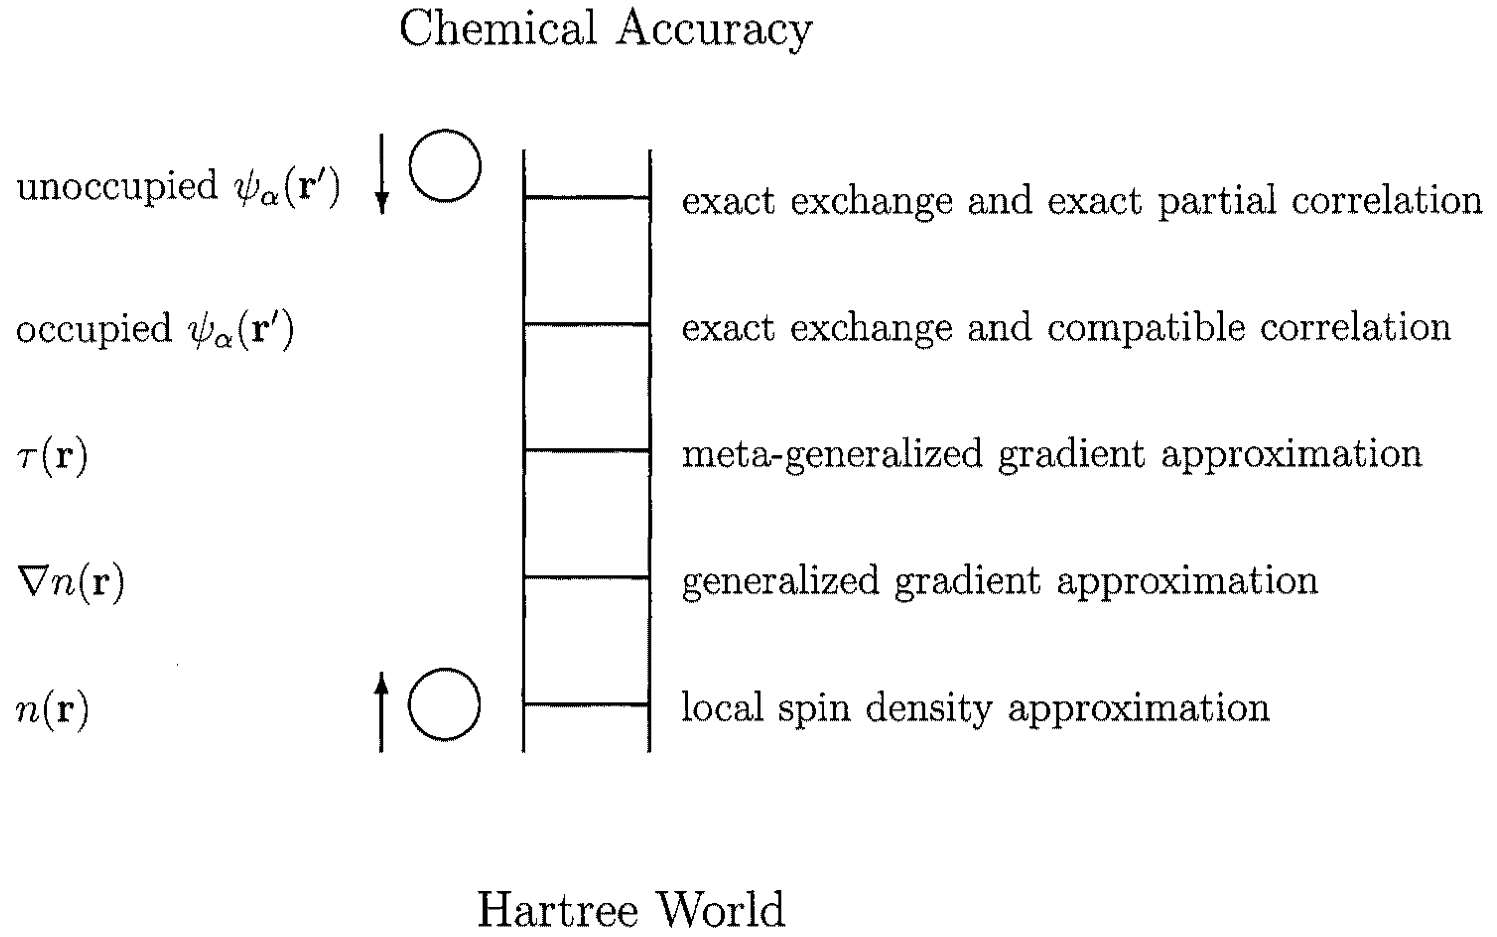
\includegraphics[width=0.6\textwidth]{fig/method/dft/jacobs_ladder.png}
	\caption{Jacob's Ladder of exchange-correlation potentials. At the lowest rung we only consider the local density. At the second rung, we include the gradient of the density. At the third, we include the kinetic energy density for the occupied orbitals $\tau (\bm{r})$, in the so-called meta-GGA functionals \cite{Tao2003}. At the fourth rung we find  Hybrid functionals which includes exact exchange and at the fifth we include both exact exchange and orbital contribtions. The original paper \cite{Perdew2001} `only guarantees safety on the two lowest rungs'. From \cite{Perdew2001}}
	\label{fig:jacobs_ladder}
\end{figure}

\subsection{The Self-Consistent Field (SCF) Cycle}
In order to actually perform a DFT calculation, we need to evaluate the Kohn-Sham equations. The solution to \eqref{eq:kohn_sham} depends on the density and gives the one-electron orbitals $\phi_i$, but at the same time the density is defined with respect to the orbitals, equation \eqref{eq:electron_density}. For this reason, the Kohn-Sham equations are solved with the Self-Consistent Field method, where we keep performing the calculations of equation \eqref{eq:kohn_sham} until the density of successive iterations agree within some pre-defined accuracy. This procedure is outlined schematically in figure \ref{fig:scf}.

\begin{figure}
	\centering
	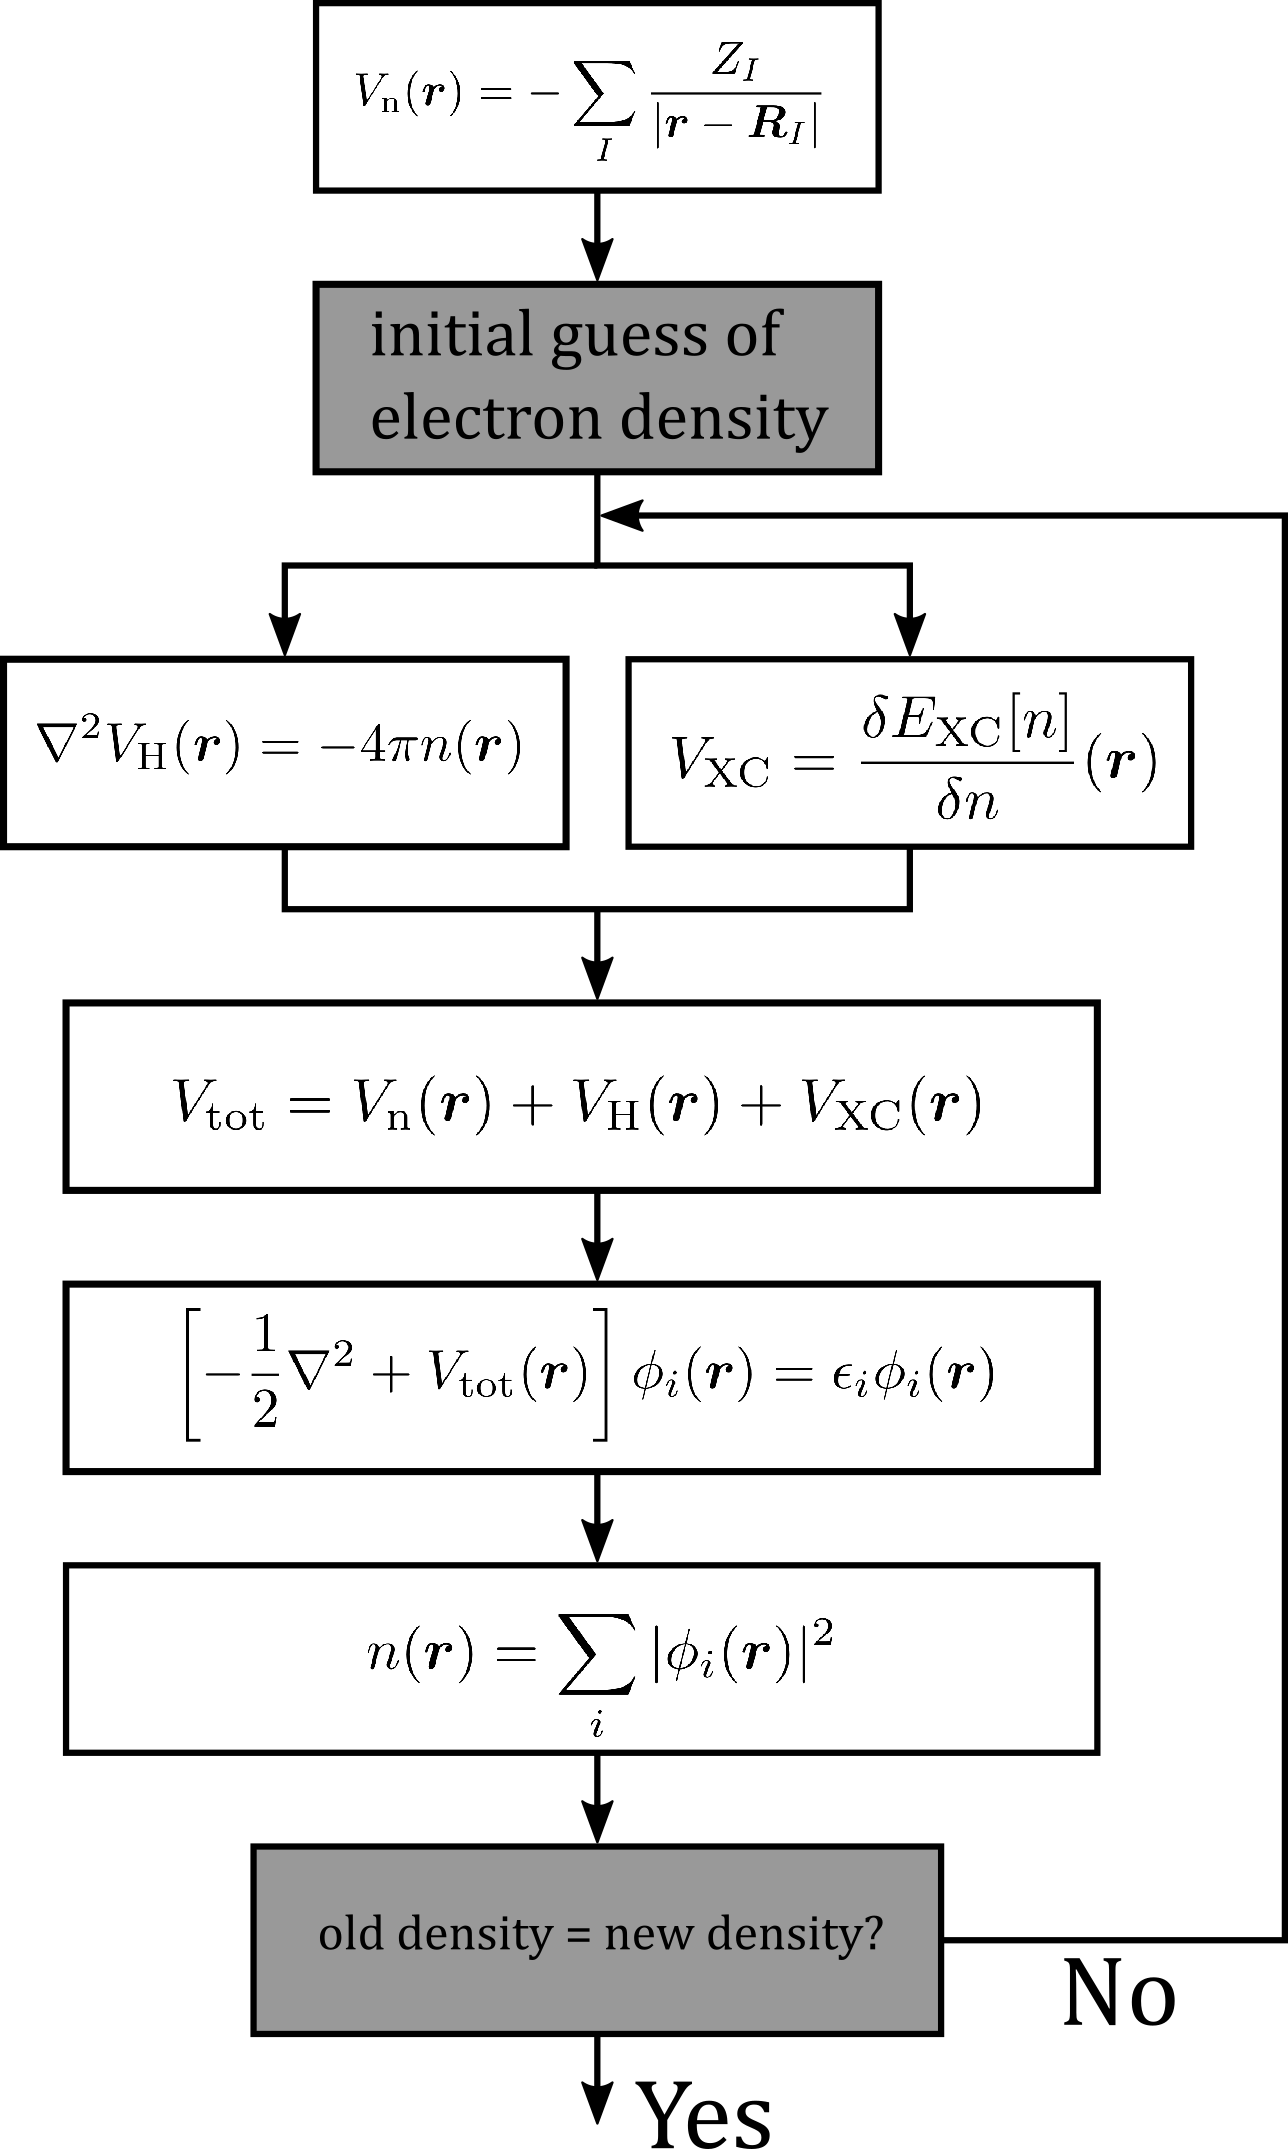
\includegraphics[width=0.4\textwidth]{fig/method/dft/scf_cycle.png}
	\caption{The self-consistent field (SCF) cycle used in most DFT calculations. $V_\text{n}$ is a fixed quantity due to the fixed nuclei approximation and will not change during the SCF cycles. The Hartree $V_\text{H}$ and exchange-correlation $V_\text{XC}$ potentials are updated throughout the run due to a change in density and finally the orbitals and electronic density is computed. This is performed until the successive iterations agree on the density. From \cite{Giustino2014}.}
	\label{fig:scf}
\end{figure}

The initial guess of the electron density is typically generated as a superposition of atomic charge densities, but can also be supplied to the program from a previous run, significantly speeding up calculations on continuation jobs. Once again, there are many subtleties regarding the actual computation of the different steps in figure \ref{fig:scf} which are outside the scope of this thesis. We will see some of these concepts in the context of the actual calculations in chapter \ref{ch:simulation}.

\subsection{DFT+U}\label{sec:ldau}
Despite the success of DFT for many materials, it generally struggles with the so-called strongly-correlated electron systems. One prominent example of this problem is exactly the materials studied in this thesis -- the cuprates. While DFT is able to include magnetism through inequivalent spin-up and spin-down densities, LDA and GGA functionals generally fail to describe the anti-ferromagnetic ground state of La$_2$CuO$_4$. The strong correlations of the $d$-orbitals cannot be described at the orbital-independent LDA and GGA level of theory.

DFT+U is an attempt to approximately treat strong correlations of specific orbitals by introducing a non-local screened Coulomb potential. This screened Coulomb interaction $U$ is only added to a sub-system consisting of the `correlated orbitals', while the remaining orbitals are treated as normal. This results in occupied states of the correlated orbitals to be shifted by $-U/2$ while the unoccupied states are shifted by $+U/2$, essentially creating a gap with the size of $U$ \cite{Anisimov1997}. However, as we shall see in chapter \ref{ch:simulation}, the actual band gap is usually smaller since the interaction is only added to the $d$ orbitals of Cu.

While DFT+U helps us with an accurate description of Mott insulators, it departs slightly from the spirit of ab-initio simulations since we are forced to input external parameters. A different choice could be to move up a rung on Jacob's Ladder (figure \ref{fig:jacobs_ladder}), but this comes at a significant computational cost and exact exchange ignores the screened nature of $U$ \cite{Anisimov1997}.

\subsection{The Hellman-Feynman Theorem and Molecular Forces}
Until now, we have only been concerned with calculating the free energy $E$ through computations through the electronic density $n$ and the electronic orbitals $\phi_i$. Since we are interested in dynamics, we need some tools to manipulate the atomic positions, despite the fact that we are in the clamped nuclei approximation. Luckily, the Hellman-Feynman theorem \cite{Feynman1939}
%
\[ \frac{\partial E}{\partial x} = \int \phi(\bm{r})^* \frac{\partial \hat{H}}{\partial x} \phi(\bm{r}) \mathrm{d}\bm{r} \]
%
turns out to be extrordinarily helpful in this regards. Intuitively, the theorem states that any derivative of the total energy can be obtained by evaluating a matrix element constructed from the derivative of the hamiltonian $\hat{H}$. Since the atomic forces are simply derivatives of $E$ with respect to atomic postions $\bm{R}_I$, this derivative can be performed directly on the first term of equation \eqref{eq:ks_toten1}. This results in the remarkable fact that we can calculate the forces on every atom in our system from a single groundstate energy, significantly reducing the computational effort.

For our purposes, the obtained forces are then treated classically with Newton's equations of motion. This will then be used to find equilibrium structures, phonon frequencies and to generate molecular dynamics trajectories. Since phonons are of particular interest to the scope of this thesis, the next section outlines how to obtain phonon frequencies from DFT and in chapter \ref{ch:simulation} I will show the result of such computations on La$_2$CuO$_4$ in various structural and electronic phases.

\section{Phonon Calculations}\label{sec:phonon_calc}
In most textbooks (e.g. Kittel \cite{Kittel2005}), phonon calculations are exemplified by simple models in one dimension consisting of only one or two inequivalent atoms. While these models are useful for providing basic results of lattice dynamical models, the extension to realistic models requires some level of abstraction in order to be useful. In particular, it is essential to cast the problem in terms of linear algebra. In this section, I will start from the (somewhat abstract) formalism used in practice and work backwards towards a physical understanding. While software such as PHONON \cite{Parlinski1997} and Phonopy \cite{Togo2015} can be used without prior knowledge of the formalism, it is always useful to have some insights about our frequently used 'black boxes`. In order to calculate the phonon spectrum for a given system in the harmonic approximation, we require the following objects:

\begin{enumerate}
	\item Primitive unit cell and fractional atomic coordinates
	\item Symmetry operations
	\item The mass of each atomic species
	\item The force constants
\end{enumerate}

Items 1-3 are familiar to most condensed matter physicists and can usually be found in various databases. The force constants, on the other hand, contains information about interatomic forces and is not directly obtainable from experiment. For this reason, phonon calculations requires some modelling either through semi-empirical or ab-initio methods. In the following I will attempt to explain what the force constants represents and how we use them to get phonon band structures.

\subsection{Theory}
We start completely generally in one dimension with an arbitrary number of unit cells containing an arbitrary number of atomic species at equilibrium. Displacements from equilibrium positions are denoted $u(jl)$, where $l$ is the unit cell index and $j \in \{1,\dots,n\}$ is the atomic index. If we consider the displacements $u$ to be small, the total energy of our system can be expressed as a Taylor series

\[ E^\text{tot} = E_0 + \sum_{l}\sum_{j} \left. \frac{\partial E}{\partial u(jl)} \right\rvert_{r_{lj}}  + \frac{1}{2} \sum_{l,\lp} \sum_{j,\jp} u(jl) \left. \frac{\partial ^2 E}{\partial u(jl) \partial u(\jp \lp)} \right\rvert_{r_{lj}, r_{\lp \jp}} u(\jp \lp) + \dots \, , \]

\noindent where $r_{lj}$ is the equilibrium position of atom $j$ in unit cell $l$. The main approximation in phonon calculations is the so-called \emph{harmonic approximation} which ignores terms with power greater than 2 in the series. Higher-order contributions are denoted \emph{anharmonic} terms and can become important at higher temperatures (phase transitions, thermal conductivity, thermal expansion). The fact that our system is in equilibrium can be stated succinctly as

\[ \frac{\partial E}{\partial u(jl)} = 0 \, , \]

\noindent for all values of $j$ and $l$. Physically these assumptions together correspond to atoms being at rest in a parabolic (harmonic) potential. Since we are interested in  dynamics, it is convenient to consider the \emph{harmonic energy} $E$ of the system

\begin{equation}
E = E^\text{tot} - E_0 = \frac{1}{2} \sum_{l,\lp} \sum_{j,\jp} u(jl) \left. \frac{\partial ^2 E}{\partial u(jl) \partial u(\jp \lp)} \right\rvert_{r_{lj}, r_{\lp \jp}} u(\jp \lp) \label{eq:eharm}
\end{equation}

\noindent If we set $j=\jp$ and $l=\lp$, we see that the harmonic energy of a single atom has the familiar form of a harmonic oscillator $E=\frac{1}{2}Ku^2$, where $K$ is the spring constant. We define

\[ \left. \frac{\partial ^2 E}{\partial u(jl) \partial u(\jp \lp)} \right\rvert_{r_{lj}, r_{\lp \jp}} = \fc = \fcbf \]

\noindent where $\bm{\Phi}$ is the called the \emph{force constant} with respect to total energy and $\bm{\Theta}$ is the force constant with respect to bond energy. We can now write the harmonic energy as

\begin{align*}
E &= \frac{1}{2} \sum_{l,\lp} \sum_{j,\jp} u(jl) \fc u(\jp \lp) \tageq\label{eq:total_energy} \\
&= \frac{1}{2} \sum_{l,\lp} \sum_{j,\jp} u(jl) \left( \fcbf \right) u(\jp \lp) \\
&= \frac{1}{2} \sum_{l,\lp} \sum_{j,\jp} \left( - \fcb u(jl)u(\jp,\lp) + \fcb u(jl)^2 \right) \\
&= \frac{1}{2} \sum_{l,\lp} \sum_{j,\jp} \left( - \fcb u(jl)u(\jp,\lp) +\frac{1}{2} \fcb \left( u(jl)^2 + u(\jp, \lp)^2 \right) \right) \\
&= \frac{1}{4} \sum_{l,\lp} \sum_{j,\jp} \fcb \left[ -2u(jl)u(\jp,\lp) + u(jl)^2 + u(\jp,\lp)^2 \right] \\
&= \frac{1}{4} \sum_{l,\lp} \sum_{j,\jp} \fcb \left[ u(jl) - u(\jp,\lp) \right]^2
\end{align*}

\begin{figure}
	\centering
	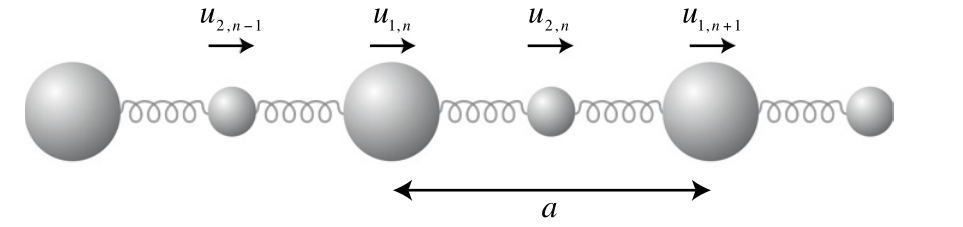
\includegraphics[width=0.9\textwidth]{fig/temp/diatomic.png}
	\caption[diatomic chain]{Diatomic chain. \todo[inline]{Make new figure. Use $l$ as unit cell index for consistency with the notation.}}
	\label{fig:diatomic}
\end{figure}

\noindent and it becomes evident that the harmonic energy can be described with respect to atoms or bonds in mathematically equivalent ways. Since the bond-centered description does not include individual atomic displacements, it is necessary to add a self-term to $\bm{\Theta}$. As a visual aid to these index-heavy equations, Figure \ref{fig:diatomic} illustrates the one-dimensional diatomic chain, which is often used in introductory texts. If we consider only nearest-neighbour interactions and identical springs, the bond-centered harmonic energy can be written

\begin{align*}
E &= \frac{1}{4} \bm{\Theta} \sum_l 2 \left[ u(1,l) - u(2,l) \right]^2 + \frac{1}{4} \bm{\Theta} \sum_n 2 \left[ u(2,l) - u(1,l+1) \right]^2 \\
&= \frac{1}{2} \bm{\Theta} \sum_l \left[ u(1,l) - u(2,l) \right]^2 + \frac{1}{2} \bm{\Theta} \sum_n \left[ u(2,l) - u(1,l+1) \right]^2
\end{align*}

\noindent where the factor of 2 comes from double-counting. The purpose of this example is to show that the (somewhat abstract) harmonic energy in equation \eqref{eq:eharm} is equivalent to our intuitive understanding of coupled harmonic oscillators. With this in mind, we can return to the matter at hand and write the equation of motion for an atom $j$ in cell $l$ through Newtons second law $F=ma$:

\[ m_j \ddot{u}(jl, t) = - \frac{\partial E}{\partial u(jl)} = - \sum_{\lp} \sum_{\jp} \fc u(\jp \lp, t) \, , \]

\noindent where $m_j$ is the atomic mass of atom $j$\todo{Where does the factor 2 come from when taking the derivative?!?}. Solutions to this equation is given as a sum of travelling harmonic waves with wave vectors $q$ and band indices $\nu \in \{1,\dots , n \}$

\[ u(jl,t) = \sum_{q,\nu} \tilde{u}(j,q,\nu) \exp (iqr(jl)) \exp(-i \omega(q,\nu) t) \, \]

\noindent where $\omega(q,\nu)$ is the frequency, $r(jl)$ is the position of atom $j$ in cell $l$ and  is the frequency and the complex number $\tilde{u}$ is called the \emph{displacement vector}. If we insert these solutions into the equations of motion and just consider one band at one wave vector we obtain

\begin{align*}
m_j \omega(q,\nu)^2 \tilde{u}(j,q,\nu) \exp(ikr(jl)) &= - \sum_{\lp} \sum_{\jp} \fc \tilde{u}(\jp,q,\nu) \exp (ikr(\jp\lp)) \\
m_j \omega(q,\nu)^2 \tilde{u}(j,q,\nu) & = - \sum_{\lp} \sum_{\jp} \fc \tilde{u}(\jp,q,\nu) \exp (ik[r(\jp\lp) - r(jl)]) \\
m_j \omega(q,\nu)^2 \tilde{u}(j,q,\nu) & = - \sum_{\lp} \sum_{\jp} \fczero \tilde{u}(\jp,q,\nu) \exp (ik[r(\jp\lp) - r(j0)]) \tageq\label{eq:motion} \, ,
\end{align*}

\noindent where the last equality is simply a change of origin in order to follow the convention of most software. The full account of phonon frequencies $\omega$ and displacements $\tilde{u}$ can be found as a solutions to equation \eqref{eq:motion}. At a given $q$ and $\nu$, the equations are indexed by $j$ and we will have $n$ equations with $n$ unknowns with respect to $\tilde{u}(j,q,\nu)$, where $n$ is the number of atoms in the unit cell. In fact, equation \eqref{eq:motion} can be written as an eigenvalue equation:

\begin{equation}
\bm{D}(q) \cdot \bm{e}(q,\nu) = \omega(q,\nu)^2 \cdot \bm{e}(q,\nu) \, , \label{eq:dynmat}
\end{equation}

\noindent where 

\[ \bm{e}(q,\nu) = \begin{pmatrix}
\sqrt{m_1}\tilde{u}(1,q,\nu) \\
\sqrt{m_2}\tilde{u}(2,q,\nu) \\
\vdots \\
\sqrt{m_n}\tilde{u}(n,q,\nu)
\end{pmatrix} \]

\noindent and the elements of $\bm{D}(q)$ are given 

\begin{equation}
D(j\jp) = \frac{1}{\sqrt{m_j m_{\jp}}} \sum_{\lp} \fczero \exp (iq[r(\jp\lp) - r(j0)]) \, . \label{eq:dynmat_ij}
\end{equation}

\noindent $\bm{D}(q)$ is known as the dynamical matrix and can be constructed solely from force constants. Furthermore, equation \eqref{eq:dynmat_ij} reveals that the dynamical matrix is Hermitian so the eigenvalues $\omega(q,\nu)^2$ are real and the eigenvectors $\bm{e}(q, \nu)$ are orthonormal. In addition, the eigenvalues and eigenvectors are trivially obtained numerically (e.g. \texttt{numpy.linalg.eigh} in the Python numpy library). In order to get the full dispersion, this diagonalization is performed for each of the $n$ bands $\nu$ at the desired wave vectors in the first Brillouin Zone (FBZ). 

The extension to 3 dimensions is done by treating the Cartesian components separately and considering $\bm{q}$ and $\bm{r}$ as vectors. The eigenvector then becomes a column vector of $3n$ components 

\[ \bm{e}(\bm{q},\nu) = \begin{pmatrix}
\sqrt{m_1}\tilde{u}_x(1,\bm{q},\nu) \\
\sqrt{m_1}\tilde{u}_y(1,\bm{q},\nu) \\
\sqrt{m_1}\tilde{u}_z(1,\bm{q},\nu) \\
\sqrt{m_2}\tilde{u}_x(2,\bm{q},\nu) \\
\vdots \\
\sqrt{m_{n}}\tilde{u}_z(n,\bm{q},\nu)
\end{pmatrix} \, , \]

\noindent the number of bands increase to $3n$ and we get a $3n \times 3n$ dynamical matrix, where each component \eqref{eq:dynmat_ij} is a $3 \times 3$ block of the form

\[
\bm{D}(j\jp) = \begin{pmatrix}
D(j\jp)_{xx} & D(j\jp)_{xy} & D(j\jp)_{xz} \\
D(j\jp)_{yx} & D(j\jp)_{yy} & D(j\jp)_{yz} \\
D(j\jp)_{zx} & D(j\jp)_{zy} & D(j\jp)_{zz}
\end{pmatrix}
\]

\noindent where

\begin{equation}
D(j\jp)_{\alpha\beta} = \frac{1}{\sqrt{m_j m_{\jp}}} \sum_{\lp} \fczero _{\alpha\beta} \exp (i\bm{q}[\bm{r}(\jp\lp) - \bm{r}(j0)]) \label{eq:dynmat_ij2}
\end{equation}

\noindent While the path was somewhat involved, it is useful to take a step back and consider the consequences of our outlined formalism. Everything we need to know about our phonon system can be obtained from the dynamical matrix that, in turn,  is constructed from force constants through equation \eqref{eq:dynmat_ij2}. Finally, all of these objects can be constructed in computationally trivial way from force constants.

\subsection{Practical considerations}\label{sec:phononpractical}
At this point, it is useful to consider how we construct elements of the dynamical matrix in practice. Inspection of equation \eqref{eq:dynmat_ij2} contains a sum over all unit cells $\lp$ and is thus an infinite sum. On the other hand, it is reasonable to assume that the dominant force constants $\bm{\Phi}$ are short range. The compromise is to use a finite supercell such that the second derivatives involved in calculating force constants outside this cell are minimized. While the reasonable size of such a supercell obviously depends on the system and model, quantum contributions to the force constants generally vanish within a distance of roughly \SIrange{10}{15}{\angstrom} \todo{CRYSTAL website reference? Maybe something better}. If the force constants can be obtained analytically from a semi-empirical potential, calculation is computationally simple and we can use large supercells. However, since force constants are usually obtained from DFT, we are limited by computational resources and are usually restricted to supercells with a maximal interatomic distance of roughly \SI{5}{\angstrom} (e.g. a cubic system with $a=\SI{10}{\angstrom}$).

Since the number of force constants needed is at least equal to the size of the dynamical matrix, the number of calculations to perform is at least $3n \times 3n$. Even for a fairly small system such as LCO in the I4/mmm space group (HTT, $n=7$) the number of elements in the dynamical matrix is $(3\cdot 7)^2 = 441$. In the finite displacement method, each force constant is the result of a self-consistent DFT calculation, so the computational effort appears prohibitively expensive at first glance. For this reason we use a numerical fitting of symmetry inequivalent force constants (see section \ref{sec:forceDFT}). In the case of LCO in the I4/mmm space group the number of necessary displacements is reduced to only 7 (6 if we ignore magnetism), making the problem much more manageable.

\subsection{Phonon eigenvectors}
The phonon dispersion is contained within the eigenvalues $\omega (\bm{q},\nu)^2$. We can plot the bands $\nu$ along high-symmetry lines in the FBZ by carefully choosing the values of $\bm{q}$ where the dynamical matrix is diagonalized. Similarly, we can sample the dispersion in a dense $\bm{q}$-mesh in order to evaluate the phonon density of states. In addition, many thermodynamic properties can be calculated by only considering the eigenvalues.

The eigenvectors $\bm{e}(\bm{q}, \nu)$ are more subtle in nature. Each component of  $\bm{e}(\bm{q}, \nu)$ is a complex number that describes the wave amplitude and phase of one atomic species $j$ in one cartesian direction $\alpha$. In addition, the eigenvector is normalized and thus only describes relative atomic motion. In order to visualize the collective displacement due to a phonon mode $\nu$ at $\bm{q}$ we can displace all atoms $j$ in unit cells $l$ by

\begin{equation}
\Delta_{jl} = \frac{A}{\sqrt{m_j}} \text{Re} \left[ \exp (i\phi) \bm{e}_j(\bm{q}, \nu) \exp (i \, 2 \pi \, \bm{q} \cdot \bm{r}(jl) \right] \label{eq:displacements}
\end{equation}

\noindent where $\bm{e}_j(\bm{q}, \nu)$ is the $j$'th component of $\bm{e}(\bm{q}, \nu)$ and $A$ is an arbitrary amplitude. The phase $\phi$ describes periodic motion of atoms. An animation can be produced by varying $\phi$ between 0 and $2 \pi$.

In \texttt{Phonopy} the eigenvectors are always given with respect to the primitive unit cell and the 3 Cartesian components are along the basis vectors of this primitive unit cell. If we want, for example, to visualize the bond-stretching mode in the HTT phase of LCO at $q=(\frac{1}{4},\frac{1}{4},0)$ in orthorhombic notation, we look at atoms in primitive unit cells with origin (0,0,0), (1,0,1), (2,0,2) and (3,0,3) using the eigenvectors at $q=(0.125,-0.125,0.125)$. For this specific mode, the movement of oxygen with fractional coordinates (0.5,0,0.5) dominates. The movement is exactly along the Cu-O bond and we can plot it in one dimension. Figure \ref{fig:bs-displacements} shows this phonon mode at the zone center, the zone boundary and halfway through the zone (where the giant phonon anomaly is observed).

\begin{figure}
	\centering
	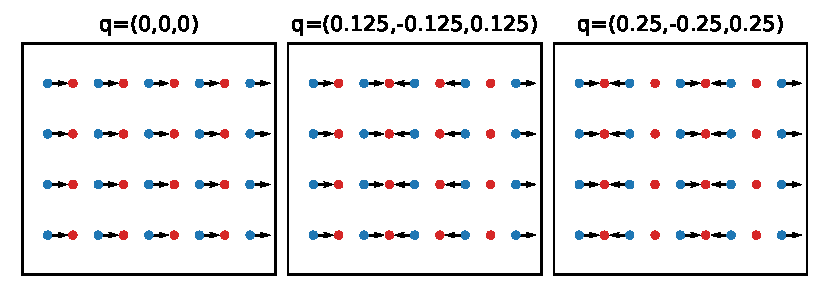
\includegraphics{fig/temp/bs-phonons.pdf}
	\caption[bond-stretching phonons visualized]{Cu-O bond stretching mode in LCO at three different values of $q$ referring to the primitive HTT (I4/mmm) unit cell. Blue markers are oxygen and red markers are copper. The phase is set to $\phi=\frac{3}{4}\pi$ in equation \ref{eq:displacements} in order to get displacement vectors of equal length.}
	\label{fig:bs-displacements}
\end{figure}

\subsection{Obtaining Force Constants from DFT}\label{sec:forceDFT}
Force constants from DFT are found in a surprisingly simple way. In the previous sections we defined the force constant with respect to total energy as

\[ \fc  _{\alpha \beta} = \frac{\partial ^2 E}{\partial u_\alpha (jl) \partial u_\beta (\jp \lp)} = - \frac{\partial F_\beta (\jp \lp)}{\partial u_\alpha (jl)} \]

\noindent where $F_\beta (\jp\lp)$ is the force on atom $(\jp \lp)$ in the direction $\beta$. Notice that everything is now labelled by a Cartesian direction and these directions are treated individually. In practice the Cartesian directions correspond to the unit cell vectors, but to reduce confusion we use the labels ($x,y,z$). We can approximate the derivative by performing a finite displacement $\Delta u_\alpha(jl)$ and simply taking the numerical derivative


\begin{equation}
\fc _{\alpha \beta} \approx - \frac{F_\beta (\jp \lp; \Delta u_\alpha (jl)) - F_\beta (\jp\lp)}{\Delta u_\alpha (jl)} \label{eq:finite}
\end{equation}


\noindent where $F_\beta (\jp\lp;\Delta u_\alpha (jl))$ is the force on atom $(\jp \lp)$ in the direction $\beta$ after performing the displacement $\Delta u_\alpha (jl)$. At equilibrium we assume $F_\beta (\jp \lp) = 0$ and we only need to calculate the forces due to a finite displacement. In ab-initio methods, there is no reason to assume a particular shape of the potential energy landscape and we can only expect the harmonic approximation to be valid for small finite displacements. For this reason, displacements have to be chosen large enough so that we are not subject to numerical noise and small enough to avoid anharmonic contributions. In \texttt{Phonopy} the default value is \SI{0.01}{\angstrom}, while \texttt{PHONON} uses \SI{0.03}{\angstrom}.

As mentioned in section \ref{sec:phononpractical}, we need a large number of force constants to construct the dynamical matrix, even when dealing with small systems. For this reason, a numerical fitting of forces and displacements, known as the Parlinski-Li-Kawazoe method \cite{Parlinski1997}, is used to find force constants. We notice that equation \eqref{eq:finite} can be written as a matrix equation for one pair of atoms $(jl)$ and $(\jp \lp)$:

\[ \bm{F}(\jp \lp) = -\bm{U}(jl) \bm{P} (jl;\jp \lp) \, , \]

\noindent where

\[ \bm{F}(\jp \lp) = (F_x \quad F_y \quad F_z) \, , \]

\[ \bm{U}(jl) = \left( \Delta u_x(jl) \quad \Delta u_y(jl) \quad \Delta u_z(jl) \right)  \]

\noindent and

\[ 
\bm{P} (jl;\jp \lp) = 	
\begin{pmatrix}
\Phi_{xx} & \Phi_{xy} & \Phi_{xz} \\
\Phi_{yx} & \Phi_{yy} & \Phi_{yz} \\
\Phi_{zx} & \Phi_{zy} & \Phi_{zz} 
\end{pmatrix}
\]

\noindent If we perform $m$ finite displacements, we get $m$ simultaneous equations for each pair of atoms:

\begin{equation*}
\begin{pmatrix} \bm{F}_1(\jp\lp) \\ \bm{F}_2(\jp\lp) \\ \vdots \\ \bm{F}_m(\jp\lp) \end{pmatrix} =
- \begin{pmatrix} \bm{U}_1(jl) \\ \bm{U}_2(jl) \\ \vdots \\ \bm{U}_m(jl) \end{pmatrix} \bm{P}(jl;\jp \lp) \, .
\end{equation*}

\noindent which can be solved by a Moore-Penrose pseudo-inverse matrix (in Numpy: \texttt{numpy.linalg.pinv}) given a sufficient number of displacements. Since $\bm{U}$ only depends on $(jl)$, we can build up the full force constant matrix by iterating this procedure over $(\jp \lp)$. The minimum number of displacements is equal to the number of non-equivalent atoms in the crystal primitive unit cell multiplied by a number of independent x,y,z coordinates in the site symmetry of a given atom \cite{Parlinski1997}. For this reason, software such as \texttt{Phonopy} and \texttt{PHONON} determines the primitive unit cell, the supercell expansion matrix and all the symmetry operations before generating displacements.

\section{Molecular Dynamics}\label{sec:method_md}
The objective of a molecular dynamics simulations is to generate a \emph{trajectory} of atomic positions as a function of time. This method has a rich history in materials science since it can be use to study ensembles explictely. The general idea is to build a real space model containing particles and their interactions and then integrate the Newtons equations of motion for this many-body system. By analyzing the resulting trajectory, one can obtain information about thermodynamic, structural and (of course) dynamical properties.

In the context of this thesis, the forces for our simulation is obtained through a DFT calculation, so that every configuarion of atomic postions requires a self-consistent calculation. For this reason, the forces are obtained ab-initio and we only have to worry about integrating the equations of motion. This can be done very efficiently using the Verlet algorithm \cite{Verlet1967}:
%
\[ \bm{r}_i(t+\Delta t) = - \bm{r}_i(t-\Delta t) + 2 \bm{r}_i(t) + \bm{a}_i (t) \Delta t^2 + \mathcal{O}(\Delta t^4) \, \]
%
where $\bm{r}_i$ is the position of atom $i$, $\bm{a}_i$ is the acceleration, $\Delta t$ is the time step. This equation can easily be obtained by summing the Taylor expansions of $\bm{r}_i(t+\Delta t)$ and $\bm{r}_i(t-\Delta t)$. The time step is a crucial choice for any MD simulation. On one hand, it is important to have a small enough time step such that the dynamics are accurately described. On the other hand, if the total simulation time is too short, we might not probe a large enough part of phase space to make the ensemble averages represenatative. In other words, short simulation times might trap you in a local minimum of phase space.

MD simulations are, unlike DFT ground state calculations, generally performed at finite temperatures. Generally this temperature is initialized by giving every atom an initial velocity taken from the Boltzman distributon at the initial temperature. During the simulation, the temperature can be controlled in different ways, depending on the thermodynamic ensemble one wishes to simulate. While energy should be conserved, the Verlet algorithm might cause the total energy to drift, especially if the system is out of equilibrium. For this reason, it is usually desirable to have a thermostat that controls the temperature. For the simulations performed in this thesis, we use the Nos\'e-Hover thermostat \cite{Nose1984}. I will not repeat the details here, but the general idea of MD thermostats is to scale the velocities such that the temperature is kept constant.

After having performed a MD simulation, we want to be able to compare with experiment. The trajectories can be analyzed in a variety of ways, but there are a few basic observables that are easy to compute in the case of crystalline materials: The phonon density of states and the pair-distribution function.  In the following, I outline how these observables are obtained in practice.

\subsection{VACF and gDOS}
It turns out \cite{Dove1993} that the phonon density of states can be found from the power spectrum of the mass-weighted velocity autocorrelation function (VACF). The VACF is, as the name implies, an expression of the correlation between velocites at different. In liquids, the VACF will rapidly decay to zero and in solids the VACF will fluctuate due to coherent vibrations around equilibrium positions. The VACF for a single atomic species $\alpha$ is defined as

\[ C_\alpha(t) = \frac{1}{3} \langle \bm{v}_\alpha(t_0) \cdot \bm{v}_\alpha(t) \rangle \]

\noindent By invoking ergodicity, the ensemble average can be replaced with a time average with respect to $t_0$.

\[ C_\alpha(t) = \frac{1}{3} \frac{1}{T-t} \sum_{t_0=0}^{T-t} \bm{v}_\alpha(t_0) \cdot \bm{v}_\alpha(t_0 + t) = \frac{1}{3} \frac{1}{T-t} \sum_{t_0=0}^{T-t} \sum_{\beta=x,y,z} v_{\alpha\beta}(t_0) v_{\alpha\beta}(t_0 + t) \]

\noindent where $T$ is the total simulation time and $v_{\alpha\beta}$ is the velocity of atom $\alpha$ in direction $\beta$. The total VACF is defined as

\[ C(t) = \sum_\alpha m_\alpha C_\alpha(t) \]

\noindent where $m_\alpha$ is a weight depending on the atomic species and the terms of the sum are the \emph{partial} VACFs. To get the mass-weighted VACF $m_\alpha$ is equal to the atomic weight of species $\alpha$ divided by the average weight of atomic species. The density of states is obtained as the power spectrum of the mass-weighted velocity autocorrelation function:
%
\[ \text{DOS}(\omega) = \sum_\alpha w_\alpha \frac{1}{2\pi} \int^{+\infty}_{-\infty} \mathrm{d}t \exp[-i\omega t] m_\alpha C_\alpha(t) \, , \]
%
where the terms of the sum, once again, determines the \emph{partial} density of states for atomic species $\alpha$. To get the neutron-weighted DOS, we set $w_\alpha$ equal to the coherent neutron cross-section of species $\alpha$. In practice both the VACF and DOS is found numerically by FFT methods.\todo{some details on this since I actually did it myself}

\subsection{Radial distribution function}

\begin{figure}
	\centering
	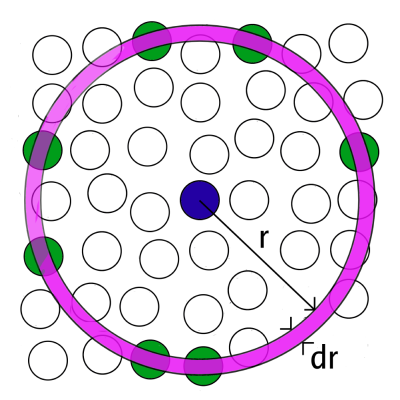
\includegraphics[width=0.4\textwidth]{fig/temp/gr.png}
	\label{fig:rdf}
	\caption[RDF visualization]{Visualization of the radial distribution function. Centered on an atom $\alpha$ (blue), we count the number of atoms $\beta$ (blue) that can be found in a spherical shell at a distance $r$ with a with $\mathrm{d}r$. As shown in the text, this can be used to construct the radial distribution function $g(r)$.}
\end{figure}

The radial distribution function is defined as
%
\[ g(r) = \frac{\rho(r)}{\rho} \, , \]
%
where $\rho(r)$ is the particle number density at a distance $r$ from an arbitrary atomic origin and $\rho = \frac{N}{V}$ is the number density of the unit cell. A visual representation of this quantity is shown in figure \ref{fig:rdf} Formally this can be found from atomic positions
%
\[ g(r) = \frac{1}{N\rho} \left\langle \sum_i^N \sum_{i \neq j} \delta(r - r_{ij})  \right\rangle \]
%
where $i$ and $j$ are particle indices and $r_{ij}$ is the distance between particle $i$ and $j$. $N$ is the total number of particles and the brackets denote an ensemble average. Due to the delta function, this expression is not particularly useful when analysing MD trajectories of discrete particle positions. To overcome this, we define $n(r,\mathrm{d}r)$ as a function that counts the number of particles at a distance $r$ within a spherical shell of thickness $\mathrm{d}r$.
%
\begin{equation}\label{eq:g_of_r}
g(r) = \frac{2 \left\langle n(r,\mathrm{d}r) \right\rangle}{N \rho V_\text{s}(r,\mathrm{d}r)} \, ,
\end{equation}
%
where $V_\text{s}(r,\mathrm{d}r) \approx 4 \pi r^2 \mathrm{d}r$ is the thickness of the spherical shell. Due to the ergodic hypothesis, the ensemble average is replaced with a time average, so that 
%
\[ \left\langle n(r,\mathrm{d}r) \right\rangle = \frac{1}{M} \sum_{k=1}^M n_k(r,\mathrm{d}r) \, \]
%
where $M$ is the number of time steps. In practice $n_k$ is evaluated by creating a list of all particle-particle distances in the frame $k$ and generating a histogram with bin size $\mathrm{d}r$. The factor of two in equation \eqref{eq:g_of_r} comes from the fact that $n_k$ only counts each pair once.

The $g(r)$ we just defined treats all particle pairs on an equal footing. In order to compare simulations with neutron scattering data it is necessary to weigh distinct particle pairs by the product of their neutron cross sections. First, we define the partial radial distribution function $g_{\alpha\beta}(r)$ as the probability of finding a particle with label $\beta$ at a distance $r$ away from a particle with label $\alpha$ plus the probability of finding a particle with label $\alpha$ at a distance $r$ away from a particle with label $\beta$.
%
\begin{align*}
g_{\alpha\beta}(r) &= \frac{ \left\langle n_{\alpha\beta}(r,\mathrm{d}r) \right\rangle}{N_\alpha  \rho_\beta V_\text{s}(r,\mathrm{d}r)} + \frac{ \left\langle n_{\alpha\beta}(r,\mathrm{d}r) \right\rangle}{N_\beta \rho_\alpha V_\text{s}(r,\mathrm{d}r)} \\
&= \frac{2V}{N_\alpha N_\beta} \frac{ \left\langle n_{\alpha\beta}(r,\mathrm{d}r) \right\rangle}{V_\text{s}(r,\mathrm{d}r)} \, ,
\end{align*}
%
where $N_i$ is the number and $\rho_i$ is the density of particle species $i$. The reason to define it in `both directions' is that $n_{\alpha\beta}$ is symmetric to exchange of particles. From the partial pair distribution functions, $G(r)$ can be trivially computed and optionally weighted by neutron cross sections, as we saw in section \ref{sec:neutron}:

\[ G(r) = \frac{1}{\overline{b}^2} \sum_{\alpha=1,\beta\geq\alpha} c_\alpha c_\beta \overline{b}_\alpha \overline{b}_\beta (g_{\alpha\beta}(r) - 1) \, , \]

\subsection{Atomic distance histograms}
If our MD simulations fulfils the ergodic hypothesis, it is useful to look at various distributions that can be extracted from the simulation. While a lot of this information is contained in the radial distribution function, the system studied in this thesis is not isotropic. In fact, the 2-dimensional nature of the cuprates appears to be essential for the electronic properties. By generating histograms for certain atoms, we can ask a few pertinent questions such as:
%
\begin{itemize}
	\item What is the distribution of Cu-O$_\text{eq}$ distance?
	\item What is the distribution of Cu-O$_\text{ap}$ distance?
	\item What is the distribution of octahedral tilts ($Q_1$, $Q_2$)?
	\item What is the nature of O$_\text{int}$ diffusion?
\end{itemize}
%
All of these questions are well-defined in the context of molecular dynamics trajectories, but it can be tedious for large systems to label all the relevant atoms. To overcome this, we generate pairs of atomic species based on certain conditions. For example, if we want to find pairs of Cu and O$_\text{eq}$, we loop over all Cu-O pairs and only list the pairs where the distance vector is less than $\bm{r} = (2.1, 2.1, 1)\,\si{\angstrom}$. After building the pair-lists it is trivial to generate histograms of certain distances.

Similarly, we can build the CuO$_6$ octahedra by applying the same idea to both equatorial and apical oxygen atoms. We can identify the 6 corners of the octahedron simply by checking the signs of the 6 distance vectors (e.g. the `top' apical oxygen will have a positive $z$ component). $Q_1$ and $Q_2$ can then be computed and we can generate histograms of the octahedral tilts.

Finally, we can also use these pairs to generate symmetry operations in a fairly simple way. Since we know that the octahedra have alternating tilt patterns, we can check the tilt pattern at frame 1 and generate a list of the 4 different combinations of $Q_1$ and $Q_2$ ((+,+),(+,-),(-,+),(-,-)). Applying these symmetry operations to our calculations then lets us obtain a histogram of the symmetry-adapted octahedral tilts.

\section{Comparing Simulation and Experiment}\label{sec:sim_experiment_compare}
Finally, we conclude this chapter by giving examples of how to compare the simulation methods with neutron scattering experiments. As we saw in section \ref{sec:neutron}, this thesis features 3 types of neutron measurements.

\begin{enumerate}
	\item Direct measurements of phonon bands with TAS spectroscopy
	\item Phonon density of states on powders with time-of-flight methods.
	\item PDF measurements of powders
\end{enumerate}

\noindent All of these can be compared directly with simulations in various ways, but there are some subtleties on how to perform this comparison correctly. In this section we thus treat them one at a time.

\subsubsection{Phonon bands with TAS}
The master equation for phonon scattering can be found in \cite{Squires2012} and directly relates the measured differential cross-section to the phonon band structure as we saw in section \ref{sec:specific_neutron}, equation \eqref{eq:one_phonon_sqw} (repeated here for clarity)
%
\begin{align*}
	S(\bm{Q},\nu,\omega) &= \frac{k_\text{f}}{k_\text{i}} \frac{N}{\hbar} \sum_{\bm{q}} | F(\bm{Q},\bm{q},\nu) |^2 ( n_{\bm{q}\nu} + 1) \delta (\omega - \omega_{\bm{q}\nu}) \delta(\bm{Q} - \bm{q} - \bm{G}) \\
	F(\bm{Q}, \bm{q}, \nu) &= \sum_j \sqrt{\frac{\hbar}{2 m_j \omega_{\bm{q}\nu}}} \bar{b}_j \exp \left( -\frac{1}{2} \langle | \bm{Q} \cdot \bm{u}(j0) |^2 \rangle \right) \exp [ -i(\bm{Q} - \bm{q}) \cdot \bm{r}(j0) ] \bm{Q} \cdot \bm{e}_j(\bm{q},\nu)
	\label{eq:one_phonon_sqw}
\end{align*}
%
Note that the equations have been rewritten slightly when compared to Squires \cite{Squires2012} (similar to what is presented on the Phonopy website \cite{phonopywebsite}), such that $S(\bm{Q},\nu,\omega)$ is defined separately for each phonon band. In addition, the sum in the phonon structure factor runs over atomic indices in unit cell 0, consistent with the definitions made earlier in this chapter.

By close inspection of equation \eqref{eq:one_phonon_sqw}, we realise that the information obtained by the calculation of phonon band structures provides us with all the information necessary to construct $S(\bm{Q},\nu,\omega)$. Since normalization on an absolute scale is usually not possible when performing a TAS experiment, we can set $N k_\text{f} / k_\text{i} = 1$ to simplify.

The $\delta$-functions in equation \eqref{eq:one_phonon_sqw} tells us that a neutron measurement will only have intensity if we measure at values of $\bm{Q}$ and $\omega$ that correspond to a point of the dispersion of band $\nu$. We thus reduce our calculations to sampling $S(\bm{Q},\nu,\omega)$ at ($\bm{q},\omega_{\bm{q}\nu}$). The only computationally heavy part then becomes the Debye-Waller factor
%
\[ W = \frac{1}{2} \left\langle | \bm{Q} \cdot \bm{u}(j0) |^2 \right\rangle \]
%
which has to be sampled at some finite grid in unit cell 0 in order to get a reasonable estimate of the ensemble average. In many cases we compare measurements to a phonon dispersion in the first BZ where $W$ varies only slightly, so if we want to sample a large number of $\bm{Q}$-points it can be advantageous to simply omit the Debye-Waller factor. As of this writing, this is not possible in Phonopy directly, so we have to live with someone heavy computations for now.

With these equations in mind, we can now plot the neutron-weighted phonon bands and compare them with TAS-measurements. We can represent the neutron weighted bands either by colouring the band-structure lines according to intensity or by giving the dispersion curves a finite Gaussian width to replicate a finite instrument resolution and/or linewidth broadening. Figure \ref{fig:bands_sqw_color_line} shows examples of the two kinds of representations. By adding obtained neutron data to these plots, we can then directly compare theory and experiment. We note here that a comparison with MD simulations is not possible since these simulations give no information about the discrete phonon bands.

\begin{figure}
	\centering
	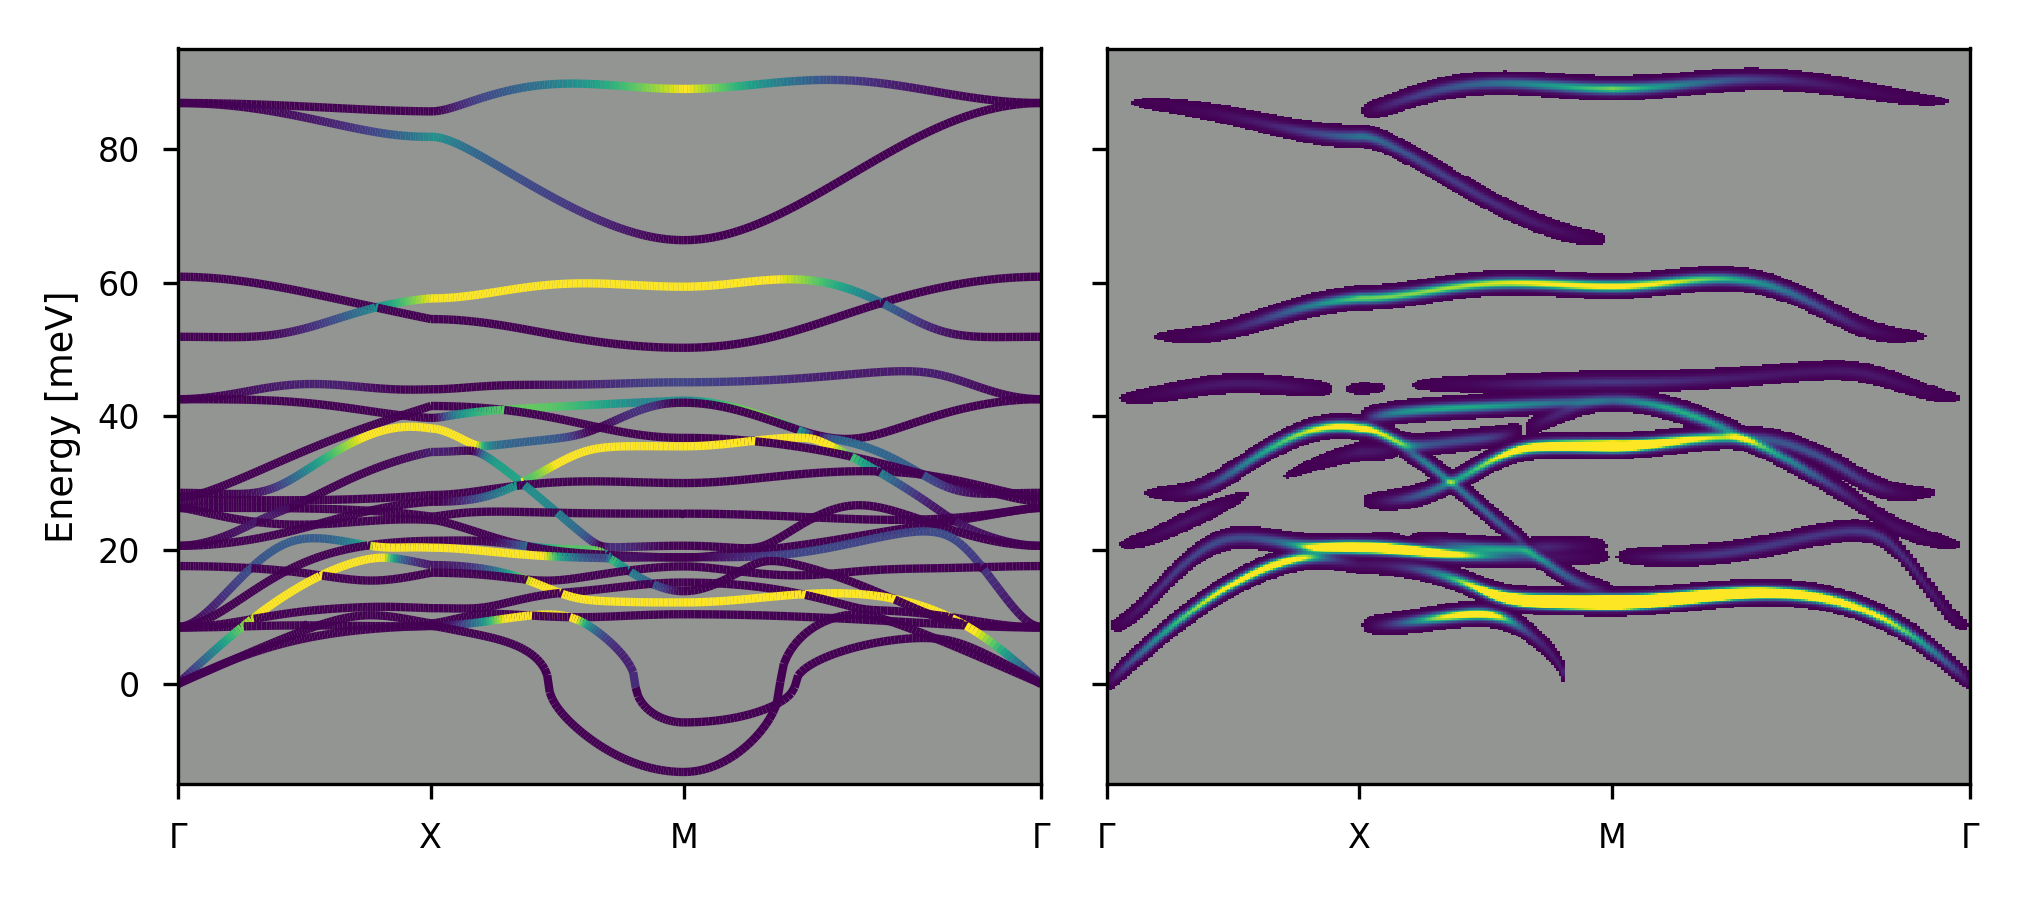
\includegraphics[width=\textwidth]{fig/method/colorbands_example.png}
	\caption[Neutron weighted bands example]{Neutron weighted phonon band structure of La$_2$CuO$_4$ in the high-temperature tetragonal phase. On the \textbf{left}, the bands are shown as a line plot where the lines are colored according to neutron intensity. On the \textbf{right} the same simulation is shown, but the bands are given a Gaussian width along the energy axis of $\sigma = \SI{0.5}{\milli\eV}$, giving a better idea of what the measured neutron spectrum would look like.}
	\label{fig:bands_sqw_color_line}
\end{figure}

\subsubsection{Phonon Density of States}
The phonon density of states (DOS) is a simple projection of the phonon bands onto the energy axis. While this obviously reduces the amount of information due to the reduction of dimensionality, the phonon DOS is a useful object for a couple of reasons:

\begin{enumerate}
	\item Often only powders are available for experiments and resolving bands can be difficult due to the rotational averaging.
	\item Many neutron scattering instruments are specifically designed for DOS measurements.
	\item DOS can be obtained from molecular dynamics as well as band structure calculations.
\end{enumerate}

\noindent The last point is particularly important in the case where we are working with defect structures such as oxygen interstitials. Here, the (local) symmetry is usually severely broken (often to P1 symmetry) and a phonon calculation would be prohibitively expensive. As shown in section \ref{sec:method_md}, the phonon DOS can be obtained, in the harmonic approximation, rather simply from a MD trajectory.

To obtain the DOS from a band-structure calculation, we perform an integration over a commensurate grid in the 1st BZ and project the result onto the energy axis for each atomic species $j$ in the following way:
%
\begin{align*}
	g^j (\omega) &= \sum_{\bm{\hat{n}}=\{x,y,z\}} \frac{1}{N} \sum_{\bm{q},\nu} \delta(\omega - \omega_{\bm{q}\nu}) \left| \bm{\hat{n}} \cdot \bm{e}_j(\bm{q},\nu) \right| ^2 \\
	g(\omega) &= \sum_j g^j(\omega)
\end{align*}
%
where $\hat{n}$ is the unit vector in the three cartesian directions. Comparing this equation with equation \eqref{eq:one_phonon_sqw} we notice that we only need to weigh by mass and the neutron cross-section in order to go from the true density of states $g(\omega)$ to the neutron $S(\omega)$\todo{look over these details once more}. If we performed a TAS experiment on a single crystal with perfect resolution at every relevant $(\bm{q},\omega_{\bm{q}\nu})$ point, these definitions would be correct and we could perform the integration on our massive 4-dimensional dataset. However, due to the nature of typical DOS measurements, we need to invoke the so-called \emph{incoherent approximation} and use the incoherent 1-phonon partial differential cross-section when treating the data. In practice this means using the total neutron cross sections ($\sigma_\text{tot}$) with the incoherent 1-phonon $S(\bm{q},\omega)$ as shown in section \ref{sec:specific_neutron}.

\subsubsection{Pair-density function measurements}
When performing neutron PDF measurements, it is possible to extract the normalized total neutron PDF (construction of partials require several measurements, see [XX]\todo{ref}). As such, we should be able to compare directly with the PDF as extracted from molecular dynamics as shown in section \ref{sec:method_md}. PDF from phonon band structure calculations are in principle possible since we can extract thermal displacements, but it is currently not a feature in Phonopy\todo{maybe do this? Could be interesting.}, so this analysis has not been performed here. 
